\documentclass[10pt]{report}
\usepackage[utf8]{inputenc}

%resize chapter-margins (https://tex.stackexchange.com/questions/149757/new-chapter-top-margin-is-large)
\usepackage{etoolbox}% http://ctan.org/pkg/etoolbox
\makeatletter %change catcode to edit package settings
% \patchcmd{<cmd>}{<search>}{<replace>}{<success>}{<failure>}
% --- Patch \chapter
\patchcmd{\@makechapterhead}{50\p@}{\chapheadtopskip}{}{}% Space from top of page to CHAPTER X
\patchcmd{\@makechapterhead}{20\p@}{\chapheadsep}{}{}% Space between CHAPTER X and CHAPTER TITLE
\patchcmd{\@makechapterhead}{40\p@}{\chapheadbelowskip}{}{}% Space between CHAPTER TITLE and text
% --- Patch \chapter*
\patchcmd{\@makeschapterhead}{50\p@}{\chapheadtopskip}{}{}% Space from top of page to CHAPTER TITLE
\patchcmd{\@makeschapterhead}{40\p@}{\chapheadbelowskip}{}{}% SPace between CHAPTER TITLE and text
\makeatother %change catcode back
% Set new lengths
\newlength{\chapheadtopskip}\setlength{\chapheadtopskip}{0pt}
\newlength{\chapheadsep}\setlength{\chapheadsep}{5pt}
\newlength{\chapheadbelowskip}\setlength{\chapheadbelowskip}{10pt}

%geometry setup 
\usepackage[paper=a4paper,inner=2cm,outer=2cm]{geometry} %left=4cm,right=2cm would be equivalent

%for custom numbering of sections
\usepackage{titlesec}

%set numbering to include subsubsections
\setcounter{secnumdepth}{3}
%include subsubsections in toc
\setcounter{tocdepth}{3}
%set section counter to negative one for zero-indexing chapter numbering
\setcounter{chapter}{-1}

%for nicer *st, *nd, and *rd
\usepackage[super]{nth}

%for checkmark symbol
\usepackage{amssymb}

%enables H placement specifier for figures
\usepackage{float}

%custom multiline comments
\usepackage{verbatim}

% Make the standard latex tables look so much better
\usepackage{array,booktabs}

%clickable toc
\usepackage{hyperref}
\hypersetup{
    colorlinks,
    citecolor=black,
    filecolor=black,
    linkcolor=black,
    urlcolor=black
}

\usepackage[
%  disable, %turn off todonotes
  colorinlistoftodos, %enable a coloured square in the list of todos
  textwidth=20mm, %set the width of the todonotes
  textsize=scriptsize, %size of the text in the todonotes
  ]{todonotes}

%support for graphics
\usepackage{graphicx}

%strikethrough markup
\usepackage[normalem]{ulem}

%shorthand for textbook name
\newcommand{\ad}{OOA\&D}

\title{System Development (SU)}
\author{cogitantium}
\date{Computer Science - \nth{3} semester}

\begin{document}
%titlepage geometry
\newgeometry{margin=1in}

% titlepage
\begin{titlepage}
    \thispagestyle{empty}
    \maketitle
\end{titlepage}

% set twopage margin dimensions after titlepage
\restoregeometry


\tableofcontents
%comment todolist out before printing, as it will take up a pagebreak
%\listoftodos
%\pagebreak

\chapter{Study regulation}
The student must achieve knowledge on following theories and methods:

\noindent Object-oriented modelling in analysis and design:
\begin{itemize}
    \item Modelling of context (problem domain and application domain) 
    \item Object-oriented concepts: class, object, events, structures, function, use cases, components and component architecture 
    \item UML: class diagram, state chart diagrams, sequence diagrams, use case diagrams 
\end{itemize}

\noindent Modelling with patterns:

\begin{itemize}
    \item Patterns for modelling the problem domain and the application domain 
    \item Patterns for connection of components 
    \item Including analysis patterns: item-descriptor, hierarchy, stepwise role, material, procedure. 
    \item Including design patterns: composite, layered architecture, observer, client-server, model-view-controller 
\end{itemize}

\noindent System development method:

\begin{itemize}
    \item Waterfall and model-driven development
    \item Iterative method and prototype-driven method
\end{itemize}

\noindent The student must achieve the following skills:
\begin{itemize}
    \item Be able to explain himself or herself precisely and use relevant concepts and modelling language
    \item Be able to model requirements for a system, its context and its different parts (model, functions and interfaces) 
    \item Be able to model a system design at component level and describe connections between components. 
\end{itemize}

\noindent The student must be able to use the concepts, the patterns, and the modelling language to describe a concrete system that solves a well-defined task.
\chapter{Lecture one: Introduction}

\section{Exam prerequisites and rules}

\begin{itemize}
    \item Written exam
    \item 4 hours duration
    \item Open book
    \item Computers are NOT permitted
    \item Internal censor
    \item Graded by the 7 point scale
\end{itemize}

\section{Workload}
\begin{itemize}
    \item Lectures - 24 hours
    \item Preparation - 48 hours
    \item Group exercises - 24 hours
    \item Submitted assignment - 21 hours
    \item Preparation for exam and trial exam - 33 hours
\end{itemize}

\section{System Development}
\begin{itemize}
    \item \textbf{Analysis:} Analysis and system requirements are analogous - the point is to find the unvarying requirements for a given system.
    \item \textbf{Design:} Work out a system design that has no major uncertainties.
    \item \textbf{Implementation:} Realise a specific design on a technical platform.
    \item \textbf{Method:} A guideline for working out system development activities, such as analysis, design, and implementation.
\end{itemize}

E.g. guidelines for work processes OOA\&D, and guidelines for documentation UML.

A method can be applied under different approaches, either the waterfall-method or the iterative-method. The writing of a book would be similar to the waterfall-method, as it's very hard not to write the given book sequentially.

\section{Object-Orientation}
An object is a single entity with an identity, a state, and some behaviour. An object belongs to a class.

A class is a description of a collection of objects sharing; structure, behavioural patterns, and attributes. Each class contains a set of objects - these are referred to to as objects of the class.

\subsection{Example with chair}
For a given dining-room chair some properties will relate to this object. The object will have an identity: myChair, a state: by dining table, not stuck, behaviour: bought, moved to, ... , sat down on, got up from, sold.

Seing a chair as a class, all chairs, as objects, will have some structure, namely an owner, attributes, positions, state (whether used or not). Behavioural pattern: \texttt{buy + \{move | sit down on + get up from\}* + sell}.

\subsection{Example with warehouse}
A warehouse is a large collection of articles stored in separate positions. Some way of defining positions of these articles is needed.

An article can be entered into, moved within, and removed from the warehouse. 

An article as an object, has an identity (barcode), state (placement in warehouse), behavioural properties (intake, moved around the warehouse, outtake).

Examples of classes in a warehouse could be:
\begin{itemize}
    \item Pallets
    \item Goods
    \item Boxes
    \item Employees
    \item Managers
\end{itemize}

\subsection{Example with gravel pit}
A class of materials has an identity (namely the type of material), state (current position, speed, wetness), behavioural patterns (dug up, moved to, moved from).

\begin{itemize}
    \item Tools
    \item Grading machines
    \item Pile
    \item Grain
    \item Material
    \item Rocks
\end{itemize}

You can discuss whether a box is a whole pallet or just a single box. 

If we had to model the gravel pit, we would have to decide on what kind of object we'd model the material as. As we're indifferent to the particular piece of grain, we're able to simplify the structure by granulating it into piles of a specific material. E.g. a pile of fine sand, a pile of clay, etc. These piles would then have an identifier as an identity, weight, and probably dimensions of the pile as state-information. Behavioural patterns would be piling material on, shovelling material out, etc.

\section{Objects in Analysis and Design}
\textbf{Analysis} concerns phenomena outside the computer system. Identity in this sense identifies a specific object. Behaviour are the events an object has performed or been subjected to. 

\textbf{Design} (and implementation) concerns phenomena inside the computer system. Identity is the description of how to get access to an object.
Behaviour is the operations an object can perform on request and offer to other objects.

\section{Model the Context}
Focus on an IT system and its context. The \textbf{problem domain} is then the part of a context that is administrated, monitored, or controlled by a system. The \textbf{application domain} is the organisation that administrates, monitors, or controls a problem domain. The system is contained within this application domain.

\section{Model of a problem domain}
\begin{figure}
    \centering
    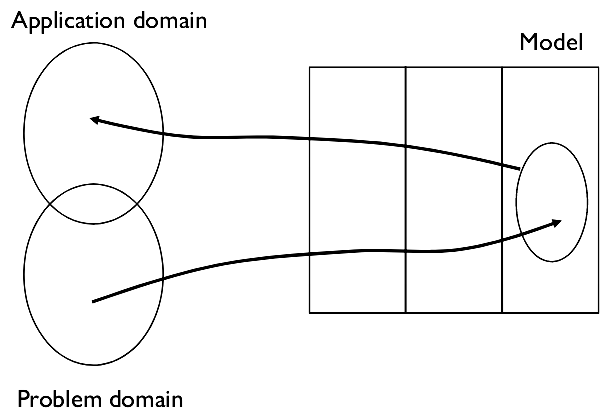
\includegraphics[width=0.6\textwidth]{figures/problemdomain.png}
    \caption{Problem domain model}
    \label{fig:problemdomainmodel}
\end{figure}

The \textbf{model}, figure \ref{fig:problemdomainmodel}, is an updated representation of the state in the problem domain. When something happens in the problem domain, e.g. a new chair is taken into a warehouse, we then register that in our model, so that it is known that we've got an extra chair. A \textbf{user} is in the application domain and gets information about the problem domain mediated through the model. 

\subsection{Example of a AAB-problem domain model}
In the application domain we've got the users that utilise the system, which presents and stores information about the team, players, and related information. The problem domain is all relevant information and actions, injuries, red/yellow cards and the like. Whenever this information changes, then a change in the model is required. Sometimes this is automated, sometimes is a manual action.

The system is then composed of a UI, which is the only thing that users see, an assorted collection of functions that transforms this data, and finally the model of the given problem domain.

\begin{figure}[h]
    \centering
    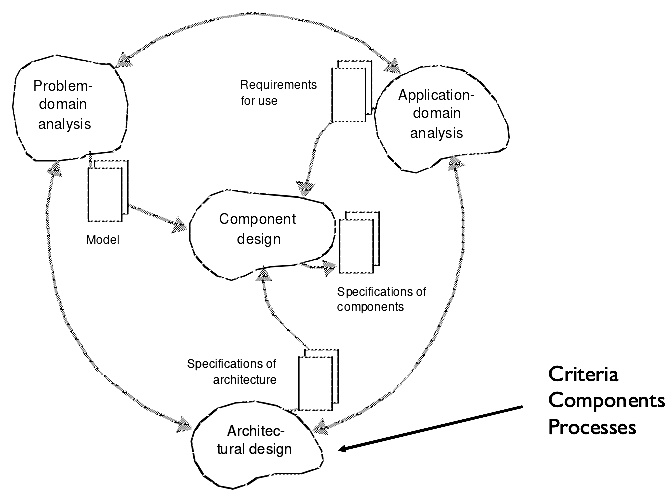
\includegraphics[scale=1.5]{figures/methodcircular.png}
    \caption{The method}
    \label{fig:methodcircular}
\end{figure}

\section{The \ad-method}
Class, structure, and behaviour relates to the problem-domain analysis. Usage, functions, and interfaces relates to the application-domain analysis. Criteria, components, and processes relates to architectural design. Lastly model component, function component, and connecting components relate component design. This is shown in figure \ref{fig:methodcircular}.

\begin{figure}[h]
    \centering
    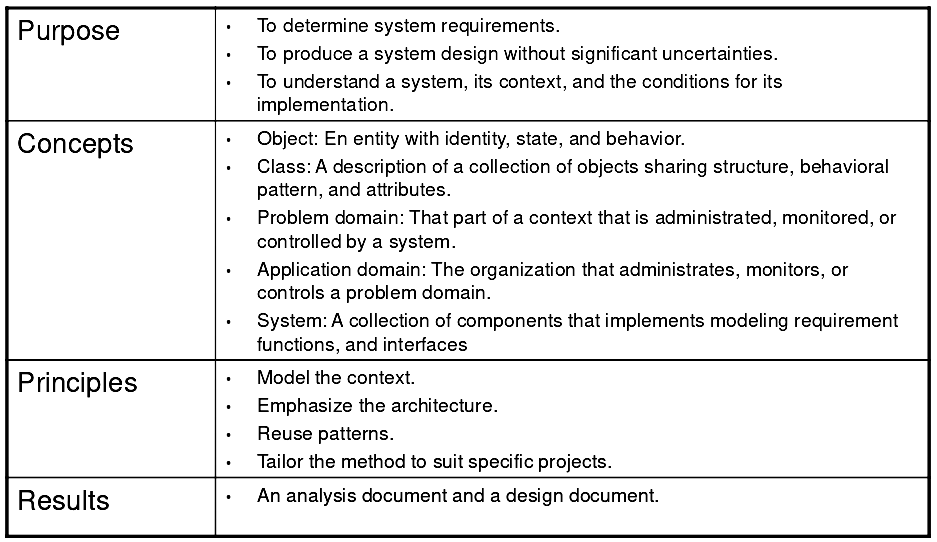
\includegraphics[width=0.75\textwidth]{figures/ooadmedthodsummary.png}
    \caption{The \ad method}
    \label{fig:methodcircular}
\end{figure}

\section{System choice}
A system definition explains all relevant areas of a given systems function and is meant to agree on the overall system characteristics. This results in a system definition that fulfils the FACTOR criterion.
The question of this activity is; \textit{should this class be included or not?}

\subsection{Situation}
Our understanding of the users' situation much be rich and abundant. In achieving this, it's important to be open and disposed toward discussion. Therefore; \textit{appreciate the situation.}

\subsection{Rich pictures}
A rich picture is an informal drawing that presents the illustrator's understanding of the situation. A rich picture focuses on the important aspects of the situation but should give a broad description of the situation that enables several alternative interpretations.

\subsection{Ideas}
Having a solid understanding of the existing situation is a good starting point for a development project. It's just as important to bring forth new ideas and ways of thinking, though.

\subsection{Create ideas}
Creating ideas can be helped with the following methods.

\subsection{Metaphors}
Imagine the user organisation or computer-system through a new lens. This helps transfer ideas and experience from other areas to the development. 

A library could be interpreted as warehouse, a supermarket, or a school through metaphors. Meaning that looking up a position, taking stock, and getting directions are similar between libraries and warehouses.

Both looking at similar and dissimilar instances of metaphors is advantageous.

\subsection{Experiments}
An experiment is a planned examination of the target solution's properties. The experience should, more or less, resemble the users' daily work.

These experiments follow the systematic approach:

\begin{enumerate}
    \item Planning
    \item Development
    \item Preparation
    \item Test
    \item Summarising
\end{enumerate}

\section{Systems}
The purpose of the third and final subactivity is to choose the actual system to develop. This is done by systematically clarifying interpretations, possibilities, and consequences of several alternative solutions. Hence, the following principle; \textit{define alternative systems.}

\section{System definition (FACTOR)}
The FACTOR criterion can be used in two ways; to either support system-definition development or describing the system and then use the criteria to see how the system definition satisfies each of the six factors. Both are equally viable.

\begin{itemize}
    \item[] \textit{Functionality:} The system functions that support the application-domain tasks
    \item[] \textit{Application domain:} Those parts of an organisation that administrate, monitor, or control a problem domain.
    \item[] \textit{Conditions:} The conditions under which the system will be developed and used.
    \item[] \textit{Technology:} Both the technology used to develop the system and the technology on which the system will run.
    \item[] \textit{Objects:} The main objects in the problem domain.
    \item[] \textit{Responsibility:} The system's overall responsibility in relation to its context.
\end{itemize}

Getting the system definition right and quick is important for all further activities. Often the system definition will iteratively be revised during \ad.

\subsection{Difficulties with system definition elements}
\textbf{Functionality and responsibility} is quite similar, however, functionality are the means to achieve the responsibility of a given system. In the greenhouse-example, updating and recording temperature versus display or control.
\textbf{Technology and conditions.} Technology is the actual tech used to develop the system and the hardware that the system will run on. Conditions are quite simply under which restraints, and conditions are this development made, e.g. in collaboration with professional or with cheapest possible hardware.

\subsection{Understanding responsibilities}
The system is responsible for certain things, which the user is not - and vice versa. Although, some of these tasks can be moved between the system and user, e.g. an autopilot on a plane.

\subsection{Evaluation and choice}
It is not the system developers' job to choose a system; your job is to facilitate choice. Active negotiation between involved parties is essential, if the system is to persevere. The choice of system should be made at an early stage, which has several implications. First, later insight may lead to changes. It's important to iterate during system choice, since describing the situation and generating ideas are so tightly tied to formulating and choosing the system definition, these subactivities cannot be completed until the final choice is made. Lastly, ensure that all parties understand the implications of what they choose at this early stage.

During this process, it's important to question arguments. Always try to base arguments on documented facts, such as \textbf{rich pictures} or \textbf{prototype evaluations}. Fundamental conflicts may also exist, and they do not disappear just because we try to avoid them. Therefore; 
\begin{center}
    \textit{we must resolve conflicts or suffer the consequences}
\end{center}

\subsection{Summary}
\begin{figure}[H]
    \centering
    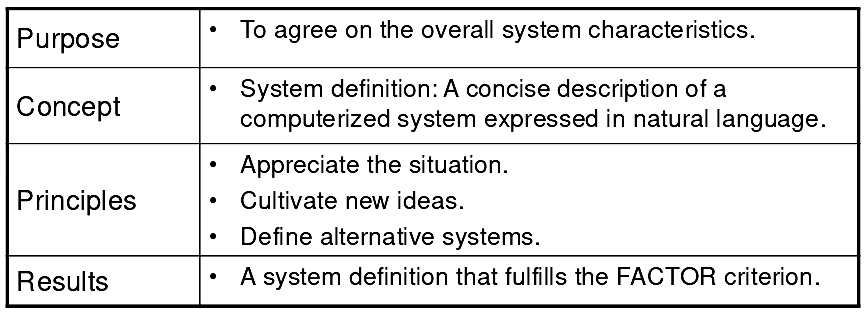
\includegraphics[width=0.75\textwidth]{figures/systemchoicesummary.png}
\end{figure}

\section{Exploring alternative system definitions}
System developers explore different alternative systems by changing elements of the system definition. E.g. with a bank, old-school banking versus modern, networked banking. Evaluate which and why the user might want either version.

\subsection{Conference administration}
Func = \textit{functionality}. Resp = \textit{responsibility}.
\begin{itemize}
    \item[Func 1] Register information about participants and produce a complete participant list
    \item[Func 2] Register general participants as well as those with an active role such as author, speaker, or reviewer. Support the administration of finances and invitations. Support development of conference programs, including registration, paper acceptance, and sessions division.
    \item[Resp 1] Support program design by producing overviews and allowing users to add components and save difference versions. Support conference operations by emphasising potential problems at regular intervals.
    \item[Resp 2] Automatic conference-planning program. Generate program from suggested sessions and incoming paper reviews.
\end{itemize}

\subsection{Principles}
\subsubsection{Appreciate the situation}
The customer's or users' understanding of the task is an important starting point. But you should also look behind their formulations and understand the situation in which the new system will be used. Rich pictures provide a quick overview of complex and ambiguous situations. They are a good basis for discussion and give us a way to express different interpretations of the same situation. 

\subsubsection{Cultivate new ideas}
Every development project is an opportunity to take a critical look at established traditions and think in new and different ways. Exemplars, metaphors, and exploratory experiments are cheap and effective techniques to bring new ideas into play.

\subsubsection{Define alternative systems}
The customer and users are responsible for choosing the solution. System definitions are brief and concise descriptions of possible alternatives that can serve as a basis for their evaluation of possibilities and their choice of a satisfactory solution.

\section{Exercises}
\begin{itemize}
    \item Write text for each element of the FACTOR criterion
    \item Introduce variations on selected elements
    \item If relevant, write the FACTOR criterion as a coherent piece of text
\end{itemize}
\subsection{Quiz}
22 minutes duration, 87\% correct answers.
\chapter{Lecture two: Classes}
\section{Problem-Domain analysis}
\begin{center}
    Principle: \textit{Model the real world as future users will see it}
\end{center}
\subsection{Results}
The first part of the results is a class diagram. This is essentially what characterises the problem domain. Some structure relations are explained in these types of diagrams.

A behavioural pattern for each class, this describes the behaviour of a class, fields, and functions.

\begin{figure}[H]
    \centering
    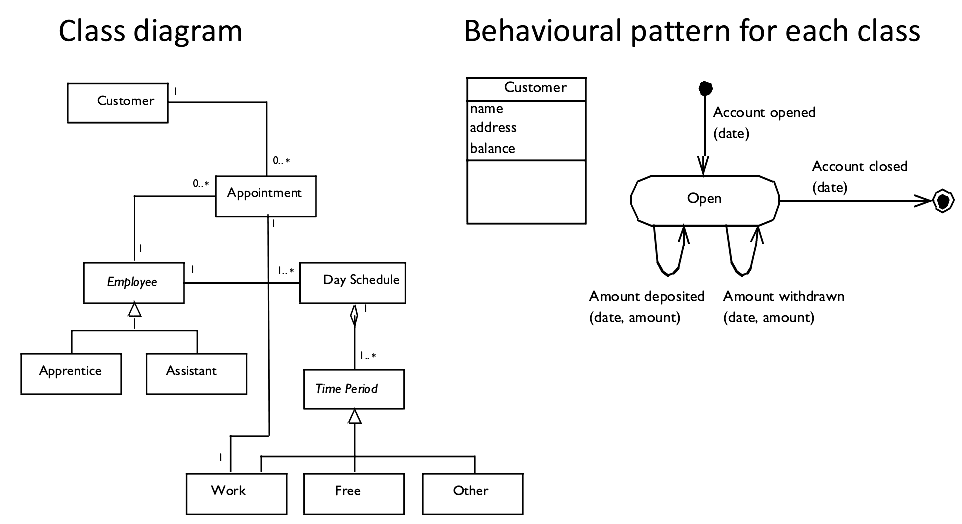
\includegraphics[width=0.75\textwidth]{figures/classdiagandbehaviouralpattern.png}
\end{figure}
\subsection{Key concepts}

\subsubsection{Problem domain}
The \textbf{problem domain} is the part of a context that is administrated, monitored, or controlled by a system. Recall that the \textbf{user} and the \textbf{system} resides in the \textbf{application domain}.

\subsubsection{The model}
The \textbf{model} is a description of classes, objects, structures, and behaviour in a problem domain. This provides an updated representation of the state in the problem domain.

In \textbf{analysis}, we describe the problem domain by an object-oriented model. In \textbf{design}, we adapt this model to become the model component of the system.

\subsection{Summary}
\begin{figure}[H]
    \centering
    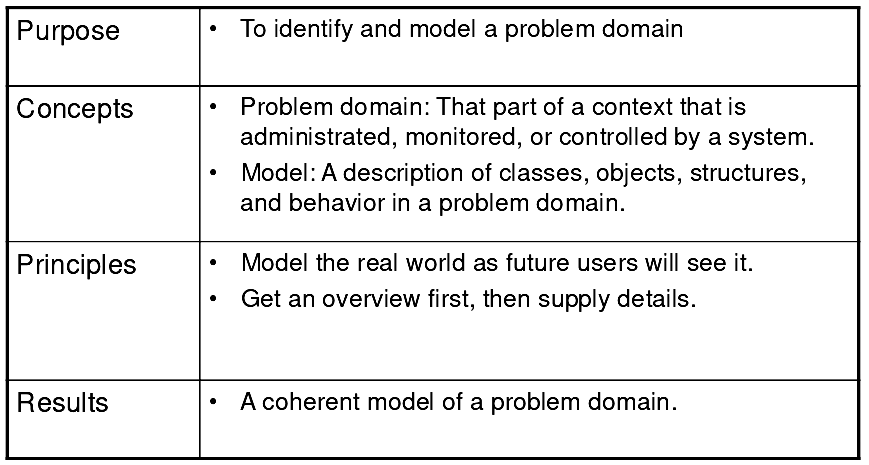
\includegraphics[width=0.75\textwidth]{figures/problemdomainanalysissummary.png}
\end{figure}
\section{The classes activity}
\subsection{Result}
An \textbf{event table}. This shows major classes and events in the problem domain. This is the starting-point for the following activity.

\begin{table}[h]
\centering
\begin{tabular}{l|l|l|l|l|l|l|l|}
\cline{2-8}
 & reserved & cancel & treated & employed & resigned & graduated & agreed \\ \hline
\multicolumn{1}{|l|}{Customer} & \checkmark & \checkmark & \checkmark &  &  &  &  \\ \hline
\multicolumn{1}{|l|}{Assistant} & \checkmark & \checkmark &  & \checkmark & \checkmark &  & \checkmark \\ \hline
\multicolumn{1}{|l|}{Apprentice} &  &  &  & \checkmark & \checkmark & \checkmark & \checkmark \\ \hline
\multicolumn{1}{|l|}{Appointment} & \checkmark & \checkmark & \checkmark &  &  &  &  \\ \hline
\multicolumn{1}{|l|}{Plan} & \checkmark &  &  &  &  &  & \checkmark \\ \hline
\end{tabular}
\caption{Event table for hair salon}
\end{table}

Shows major classes and events in the problem domain. The classes are often listed horizontally, but depends on number of each.

\subsection{Classifying objects and events in the problem domain}
We try to distil the messy real world of classes and objects and events by abstracting and classifying these. 

\subsection{Key concepts}

\subsubsection{Object and class}
An \textbf{object} is an entity with; \textbf{identity, state, and behaviour}. 

\begin{itemize}
    \item[] identity: \texttt{myChair}
    \item[] state: by dining table, free
    \item[] behaviour: bought moved to, ..., sat down on, got up from, ...., moved to, ..., sold
\end{itemize}

\noindent Two kinds of objects: 
\textbf{Analysis objects} describes phenomena outside the system, such as people and things, which are typically independent. although we cannot always command them, we must register the events they perform or experience. \textbf{Design objects} describe phenomena within the system that we can control. We describe their behaviour as operations for the computer to carry out.

\bigskip
\noindent A \textbf{class} is a description of a collection of objects sharing; \textbf{structure, behavioural pattern, and attributes}

\begin{itemize}
    \item[] structure: has an owner
    \item[] attributes: position, vacant
    \item[] behavioural pattern: \texttt{buy + \{move + | sit down on + get up from\}* + sell}
\end{itemize}

\subsubsection{Event}
An event is \textbf{an instantaneous incident involving one or more objects.} Atomic, meaning that they should not be further divisible (if so, use those subevents instead), common to several objects, and have a unique name. At IKEA this could be \texttt{payment\_completed}, when payment and maybe receipt-printing for the cart has been completed.

\subsection{Classes: Activities}
Find candidates for both classes and events, and evaluate these and select systematically. This will result in an event table.

Common techniques for generating candidate lists, e.g. brainstorming, could be to make a list of all potentially relevant classes and events. You should consider many sources; your own perception of the problem domain, existing descriptions (rich pictures, the system definition, etc.), collaboration with prospective users.

Naming must be \textbf{simple} and \textbf{readable} and should originate in the problem domain.

\noindent Classes should be found by looking for nouns, eliminate nouns that reflect administration objects and devices. Make sure to only describe a single instance (object).

\noindent Events should be found by looking for verbs, eliminate verbs related to the way users carry out their job - those related to the application domain. Make sure to only describe a single event - the concept of an \textit{atomic} event.

\subsection{FACTOR example; hair salon}
\begin{itemize}
    \item[] \textbf{Functionality: } Support for work planning and appointments
    \item[] \textbf{Application domain: } Managing customers, their treatments, and appointments, and planning employees' work schedules
    \item[] \textbf{Conditions: } Developed in close cooperation with the employees
    \item[] \textbf{Technology: } Smaller PC or Macintosh with a large graphical screen
    \item[] \textbf{Objects: } Customers, employees, appointments, and work schedules
    \item[] \textbf{Responsibility: } Tool for reliable administration and common mediator
\end{itemize}

\subsection{Classes and Events example; hair salon}
The symbols \texttt{+} and \texttt{-} specify whether lecture-discussion resulted in including or omitting the given class or event.

%latexmaster!!! :yeet:
\begin{minipage}[t]{\textwidth}
    \begin{minipage}[t]{.5\textwidth}
        \noindent Classes:
        \begin{itemize}
            \item Plan \texttt{+}
            \item Customer database \texttt{-}
            \item Appointment book \texttt{-}
            \item Cash register \texttt{-}
            \item Appointment \texttt{+}
            \item Desired vacation \texttt{-}
            \item Work schedule \texttt{-}
            \item Boss, assistant, receptionist, apprentice, customer \texttt{+}
            \item Chair \texttt{-}
            \item Salon \texttt{-}
        \end{itemize}
    \end{minipage}%
    \begin{minipage}[t]{.5\textwidth}
        \noindent Events:
        \begin{itemize}
            \item reserved \texttt{+}
            \item cancelled \texttt{+}
            \item customer arrived \texttt{-}
            \item treated \texttt{+}
            \item payment received \texttt{-}
            \item employed \texttt{+}
            \item resigned \texttt{+}
            \item graduated \texttt{+}
            \item agreed \texttt{+}
            \item material used \texttt{-}
            \item item purchased \texttt{-}
            \item customer picked up \texttt{-}
            \item arrived at workplace \texttt{-}
            \item left workplace \texttt{-}
        \end{itemize}
    \end{minipage}
\end{minipage}


\subsection{Systematic evaluation}%hov, jeg fjernede den, sry tænkte bare at highlighte - ya, rigtig god idé, synes bare det blev lidt meget når de var linebreaked, men gør det gerne!
\textbf{General evaluation criteria;} is the class or event within the system definition, and is the class or even relevant for the problem-domain model. 

\noindent \textbf{Criteria for classes;} can you identify objects from the class, does the class contain unique information, does the class encompass multiple objects, and does the class have a suitable and manageable number of events.

\noindent \textbf{Criteria for events;} is the event instantaneous, is the event atomic, and can the event be identified when it happens. 

\subsection{Summary}
\begin{figure}[H]
    \centering
    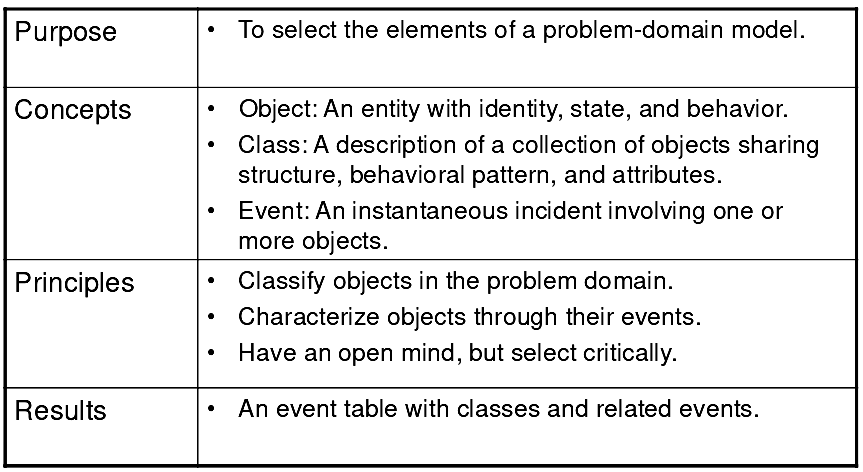
\includegraphics[width=0.75\textwidth]{figures/classessummary.png}
\end{figure}
\section{Challenges in this activity}
\begin{itemize}
    \item Classifying classes and events is mentally challenging %lol, wtf u mean Stage
    \begin{itemize}
        \item Difficult to find the right granularity
        \item Difficult to transcend the existing situation
    \end{itemize}
    \item Selecting the relevant classes and events is often difficult
    \begin{itemize}
        \item Use the criteria
        \item Be explicit about the reasoning for excluding
    \end{itemize}
    \item Functions are often described as events - but we usually do not want to register the application of a function
    \begin{itemize}
        \item Make a preliminary function list to remember them
    \end{itemize}
\end{itemize}

\section{Principles}
\subsection{Classify objects in the problem domain}
Make relevant abstractions and study reality. Focus on the problem domain and the different understandings that users have of it. Do not describe the application domain or the system itself.

\subsection{Characterise objects through their events}
Use events to understand the dynamics of the problem domain. It is the events that define the dynamic nature of objects and their mutual interplay.

\subsection{Have an open mind, but select critically}
Be open-minded and consider many candidates for classes and events. On the other hand, be critical and thorough in evaluating whether each class or event candidate is necessary in relation to the system definition.

\section{Exercises for lecture two}
\begin{itemize}
    \item Find candidates for classes
    \item Find candidates for events
    \item Select the relevant classes and events
    \item Be precise in the argumentation about which classes and events that should be included - \textit{use the criteria}
    \item Combine classes and events in an event table - \textit{which classes are involved in which events}
\end{itemize}
\subsection{Quiz}
12 minutes duration. 90\% correct answers.

\subsection{Exercise 3.6.16}
Classes:
\begin{itemize}
    \item Elevator
    \item Floor
    \item Button
    \item Passenger
    \item Request
    \item Sensors
    \item Door
    \item Call button
\end{itemize}

Events:
\begin{itemize}
    \item Door opened
    \item Door closed
    \item Button pressed
    \item Arrived at floor
    \item Floor left
    \item Elevator called
    \item Floor requested
    \item Elevator malfunctioned
    \item Light turned on
    \item Light turned off
    \item Turned on
    \item Turned off
\end{itemize}

\subsubsection{Event table}

\begin{table}[h]
\centering
\begin{tabular}{|l|l|l|l|l|l|}
\hline
 & Elevator & Floor & Button & Request & Sensor \\ \hline
Door opened & x & x &  &  & x \\ \hline
Door closed & x & x &  &  & x \\ \hline
Arrived at floor & x & x &  &  & x \\ \hline
Floor departed & x & x &  &  & x \\ \hline
Floor requested &  & x & x & x &  \\ \hline
Request fulfilled &  & x &  &  & \\ \hline
Elevator malfunctioned & x &  &  &  & x \\ \hline
Light turn on &  &  & x & x &  \\ \hline
Light turn off &  &  & x & x &  \\ \hline
Turned on & x &  & x & x &  \\ \hline
Turned off & x &  & x & x &  \\ \hline
\end{tabular}
\end{table}
\chapter{Lecture three: Structure}
\begin{comment}
\section{Problem domain analysis}

\subsection{Results}
Class diagram and behavioural patterns, or state-change diagrams for each class. 
This could possibly be done in UML.


\subsection{Key concepts}
The problem domain is the part of a context that is administrated, monitored, or controlled by a system. Examples of problem domains:
\begin{itemize}
    \item Students in a education institution
    \item Employees in a company
    \item Items in a warehouse
    \item Customers in a hair salon
    \item Movies available for streaming
\end{itemize}


\subsection{Classes: Results}

\begin{table}[h]
\centering
\begin{tabular}{l|l|l|l|l|l|l|l|}
\cline{2-8}
 & reserved & cancel & treated & employed & resigned & graduated & agreed \\ \hline
\multicolumn{1}{|l|}{Customer} & \checkmark & \checkmark & \checkmark &  &  &  &  \\ \hline
\multicolumn{1}{|l|}{Assistant} & \checkmark & \checkmark &  & \checkmark & \checkmark &  & \checkmark \\ \hline
\multicolumn{1}{|l|}{Apprentice} &  &  &  & \checkmark & \checkmark & \checkmark & \checkmark \\ \hline
\multicolumn{1}{|l|}{Appointment} & \checkmark & \checkmark & \checkmark &  &  &  &  \\ \hline
\multicolumn{1}{|l|}{Plan} & \checkmark &  &  &  &  &  & \checkmark \\ \hline
\end{tabular}
\caption{Event table for hair salon}
\end{table}

Shows major classes and events in the problem domain. The classes are often listed horizontally, but depends on number of each.

\section{Classifying objects and events in the problem domain}
Abstract and classify phenomena in the problem domain into objects and events within the requirements mentioned in earlier sections.

\section{Key concepts: Event}
An \textbf{event} is an instantaneous incident involving one or more objects. These are \textbf{atomic, instantaneous, common to several objects, and unique in name.}

Examples from IKEA:
\begin{itemize}
    \item Item received from producer
    \item Item stored in warehouse
    \item Item selected by customer
    \item Item picked in warehouse - OK?
    \item Item sold
\end{itemize}


\section{Classes: Summary}
\begin{table}[h]
\centering
\begin{tabular}{|l|l|}
\hline
Purpose & To select the elements of a problem-domain model. \\ \hline
Concepts & \begin{tabular}[c]{@{}l@{}}Object: An entity with identity, state, and behaviour.\\ Class: A description of a collection of objects sharing structure, behavioural pattern, and attributes.\\ Event: An instantaneous incident involving one or more objects.\end{tabular} \\ \hline
Principles & \begin{tabular}[c]{@{}l@{}}Classify objects in the problem domain.\\ Charaterise objects through their events.\\ Have an open mind, but select critically.\end{tabular} \\ \hline
Results & An event table with classes and related events. \\ \hline
\end{tabular}
\end{table}
\end{comment}

%old shit above
\section{Structure}
\subsection{Result}
This activity results in a class diagram.
\begin{figure}[H]
    \centering
    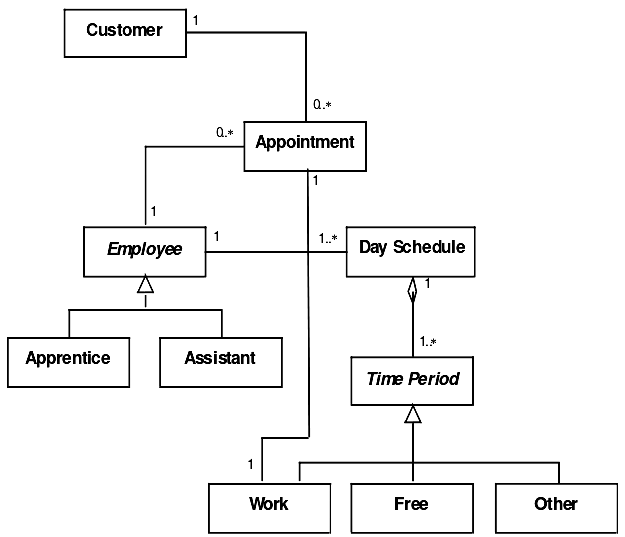
\includegraphics[width=.6\textwidth]{figures/classdiagram.png}
\end{figure}
\subsection{Key concepts}
\subsubsection{Generalisation}
Generalisation: A general class (the super class) describes properties common to a group of specialised classes (the subclasses)
Object oriented, as in a passenger car can both be a taxi and a private car. This is essentially \textbf{is-a} relations, e.g. \textit{a taxi \textbf{is-a} passenger car}. 

\begin{figure}[H]
    \centering
    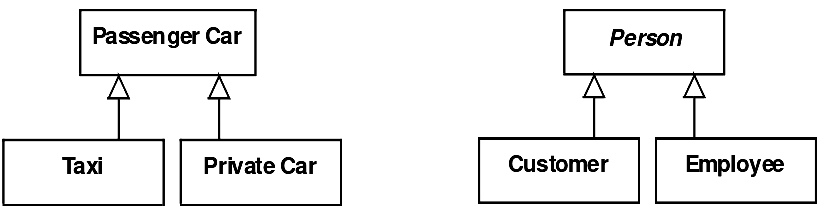
\includegraphics[scale=1.5]{figures/generalisation.png}
\end{figure}

Furthermore, there's generalisation, specialisation, and abstract classes. Abstract classes are denoted by \textit{italics}.

\subsubsection{Cluster}
A collection of related classes
\begin{figure}[H]
    \centering
    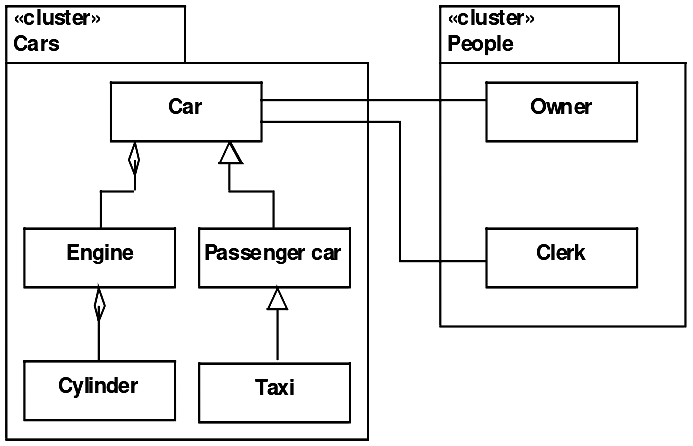
\includegraphics[scale=1.5]{figures/cluster.png}
\end{figure}

\subsubsection{Aggregation}
Aggregation: A superior object (the whole) consists of a number of inferior objects (the parts). The aggregation structure drawn with a line, and a rhomb at (the whole) class.
Physical aggregation (unusual), relations alike \textbf{has-a} or \textbf{owns-a}, these are more common. Usually on different, conceptual, levels. Typical aggregations; whole - part, container - contents, and union - member.

\begin{figure}[H]
    \centering
    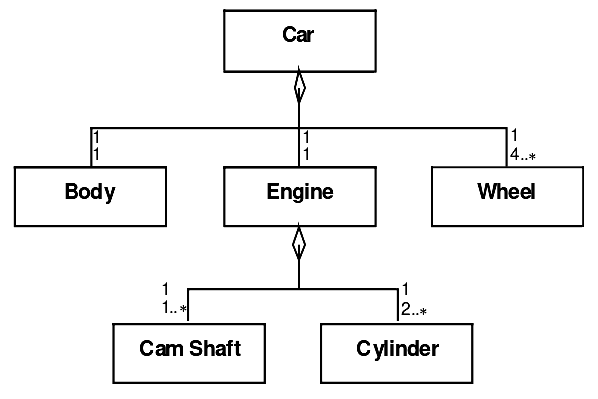
\includegraphics[scale=1.5]{figures/aggregation.png}
\end{figure}

\subsubsection{Association}
Association: A meaningful relation between a number of objects. This is often used when aggregation would imply a too strong relation. Linguistically, express association with "knows" or "associated-with".
Relations, usually a loose (non-defining) relation, usually on the same \textit{level}, and these can be named (but this is often because a class is missing, so instead of naming the association, we can introduce that class). 
\begin{figure}[H]
    \centering
    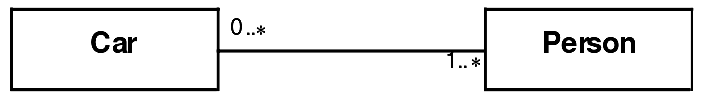
\includegraphics[scale=1.5]{figures/association.png}
\end{figure}

\subsection{Activities}
\begin{figure}[H]
    \centering
    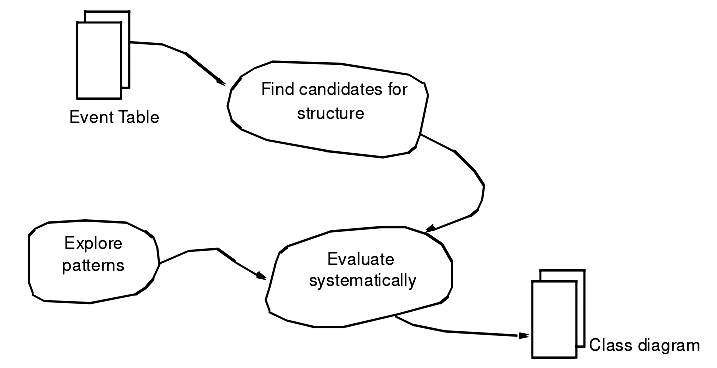
\includegraphics[scale=1.5]{figures/structureactivity.png}
\end{figure}

\subsection{Evaluate systematically}
\begin{itemize}
    \item Structures must be used correctly
    \begin{itemize}
        \item Generalisation versus aggregation (\textit{is-a / has-a})
        \item Aggregation versus association (page 87 in \ad)
    \end{itemize}
    \item Structures must be conceptually true
    \begin{itemize}
        \item Names, concepts, and structures reflect the user's understanding
        \item Especially for the prospective user
    \end{itemize}
    \item Structures must be simple
    \begin{itemize}
        \item Especially at the top levels
        \item Avoid unnecessary generalisations and aggregations
        \item Avoid objects changing class
        \item Check against the system definition
    \end{itemize}
\end{itemize}

\section{Discuss hair salon class diagram}
\begin{figure}[H]
    \centering
    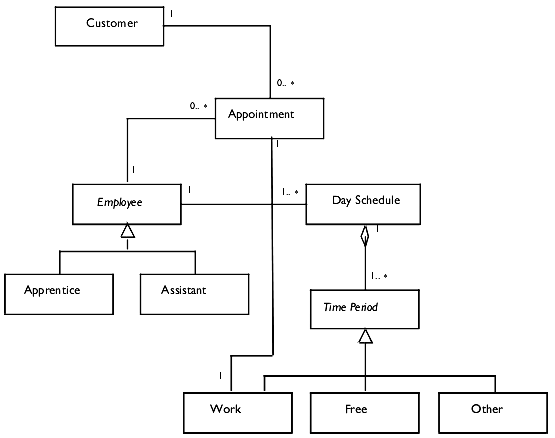
\includegraphics[width=.75\textwidth]{figures/hairsalondiscussion.png}
\end{figure}

Customer and appointment is a candidate for aggregation, as it satisfied properties specified on page 87.

\noindent The following were found during lecture discussion:
\begin{itemize}
    \item Customer - Appointment: Aggregation from Customer
    \item Appointment - Employee: OK
    \item Employee - Day Schedule: Aggregation from Employee
    \item Time Period specialisations: Different solution, e.g. remove the tree specialisations
\end{itemize}

\subsection{Summary}
\begin{figure}[H]
    \centering
    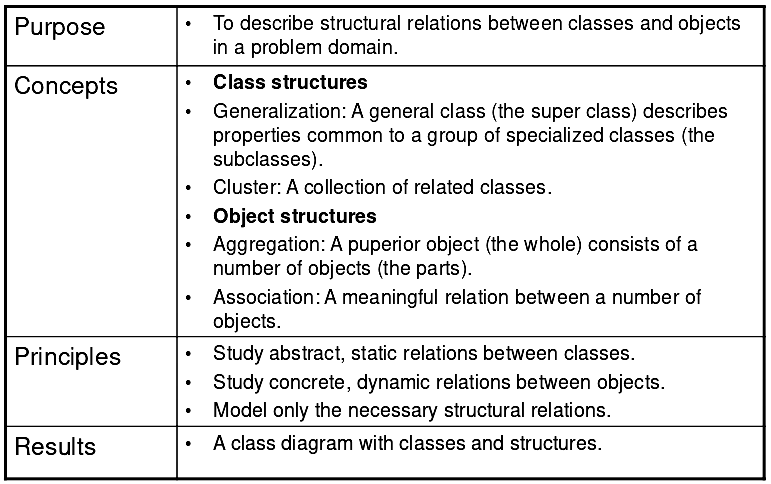
\includegraphics[scale=2]{figures/structuresummary.png}
\end{figure}

\section{Example with a streaming service}\label{structure:streamingservice}
\begin{itemize}
    \item[] \textit{Functionality:} Register the movies the customers see and the songs they listen to, and support payment by customers for their consumption of movies and songs
    \item[] \textit{Application domain:} Will be used by the administrative personnel that is employed by the organisation that provides the streaming service
    \item[] \textit{Conditions:} Developed for the administrative personnel
    \item[] \textit{Technology:} PC platform with typical tools
    \item[] \textit{Objects:} Customer, Movie, Song
    \item[] \textit{Responsibility:} Registration, administration, and payment of customers' consumption
\end{itemize}

An initial class diagram for this FACTOR:
\begin{figure}[H]
    \centering
    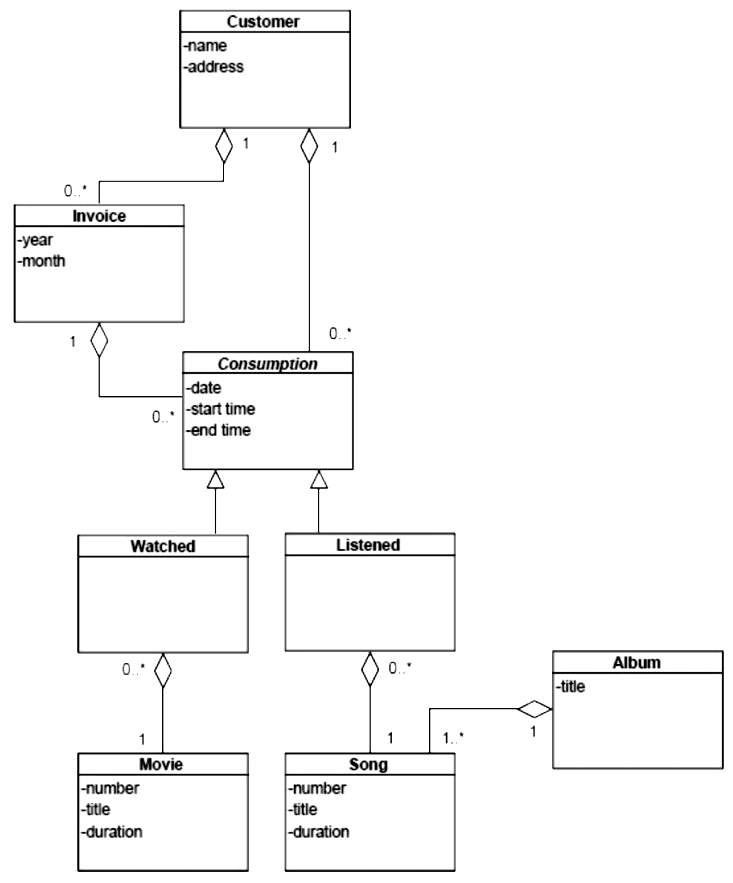
\includegraphics[width=.5\textwidth]{figures/prelimstreamclassdiagram.png}
\end{figure}

\section{Patterns}
\subsection{Role pattern}
A person can have different roles. The roles of a person change dynamically over time. Here employees and customers are generalised into persons. A person then aggregates one or more roles. If the roles have nothing in common, we use a simplified pattern without the role class, with the employee role and customer role directly aggregates to person.

\begin{figure}[H]
    \centering
    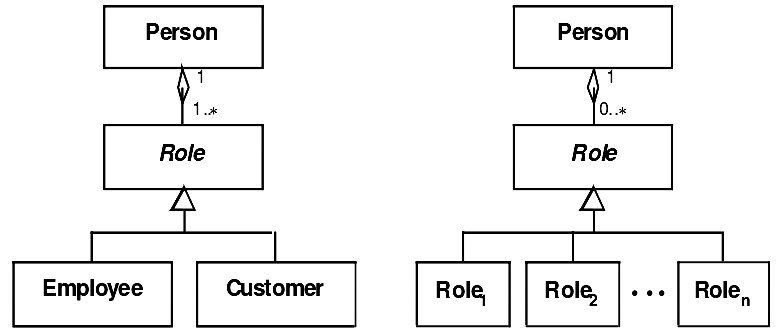
\includegraphics[width=.5\textwidth]{figures/rolepattern.png}
\end{figure}

\subsection{Relation pattern}
The purpose of the pattern is to relate two parties to each other. Two variations; In the first, both of the related parties aggregate the relation object. This indicates that they both own the relation. Second variation is both parties connect to the relation with association. This indicates a loose relation.

\begin{figure}[H]
    \centering
    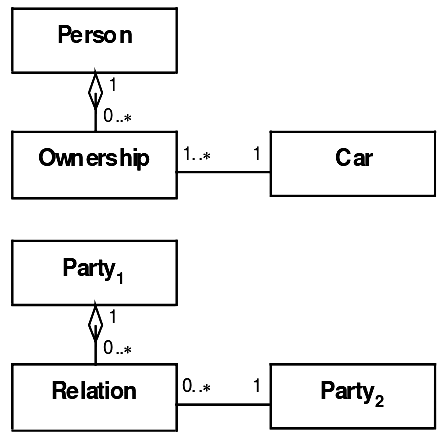
\includegraphics[width=.35\textwidth]{figures/relationpattern.png}
\end{figure}

\subsection{Hierarchy pattern}
When using this pattern, we must decide what the elements are and how many levels of hierarchy to organise them in. In chapter 19, an advanced application of this pattern is shown in the "Program" cluster of the conference planning system. A useful variation on this pattern, is where objects on one level, can belong to several objects on the level above. 

\begin{figure}[H]
    \centering
    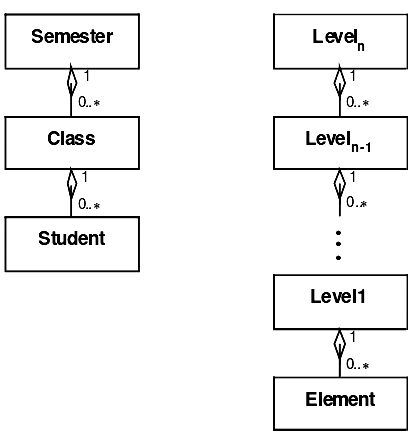
\includegraphics[width=.4\textwidth]{figures/hierachypattern.png}
\end{figure}

\subsection{Item-descriptor pattern}
Properties of objects from one class (items) are described in an object from another class (descriptor). An object from the overall class "Descriptor" defines specific properties shared by all the related objects from the "Item" class. This pattern is useful in systems that administrate different kind of descriptions, such as contracts, insurance policies and so on.

\begin{figure}[H]
    \centering
    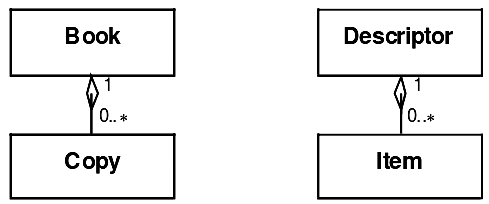
\includegraphics[width=.4\textwidth]{figures/itemdescriptorpattern.png}
\end{figure}

\section{Challenges}
\begin{itemize}
    \item Selecting the right structure is difficult
    \begin{itemize}
        \item Try them out one-by-one for each pair of classes
        \item Use the criteria to select the most correct structure.
    \end{itemize}
    \item It is very easy to include too many structures
    \begin{itemize}
        \item Try to simulate functions and see if you can get to the relevant objects.
    \end{itemize}
\end{itemize}

\noindent A good test is to try out functions and notice if any objects are not relevant.

\section{Principles}
\subsection{Study abstract, static relations between classes}
We use generalisation and cluster structures to describe static, conceptual relations between classes. Generalisation structures express different levels of abstraction in our model, while we use clusters to achieve clarity.

\subsection{Study concrete, dynamic relations between objects}
We use aggregation and association structures to describe dynamic, concrete relations between objects. Aggregation structures describe superior objects as consisting of or containing subobjects, while association structures describe other meaningful relations between objects.

\subsection{Model only the necessary structural relations}
The model should describe only the structural relations that are necessary to satisfy the system definition. In general, the model should focus on the important aspects and contain a minimal number of structural relations. 

\section{Exercises for lecture three}
\begin{itemize}
    \item Find candidates for structural relations between the classes in your event table - \textit{do this in pairs}
    \item Explore if any of the patterns are relevant to your case - \textit{do this for each class}
    \item Make a class diagram
    \item Look for opportunities to simplify and extend the class diagram
\end{itemize}
\subsection{Quiz}
92\% correct over 8 minutes.

Object structure and role-patterns had errors in the quiz.
\chapter{Lecture four: Behaviour}
\section{Behaviour}

\subsection{Result}
The result of this activity is a schematic of behavioural paths.

\begin{figure}[H]
    \centering
    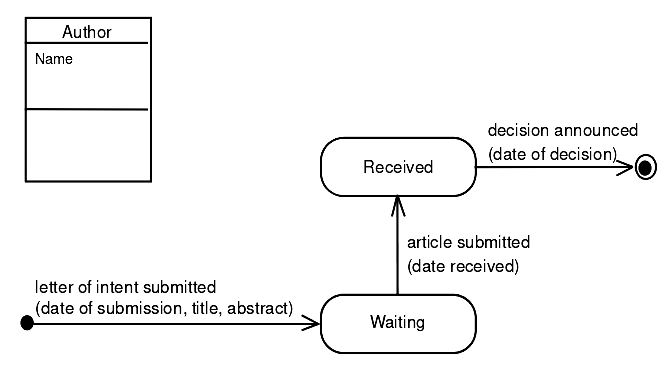
\includegraphics[width=.6\textwidth]{figures/behaviourresult.png}
\end{figure}

\subsection{Activities}

The behaviour activity includes four activities. Start with event table and class diagram. We start with describing behavioural patterns for each class, using related events. General patterns of class behaviour are used to improve description and discover new ways of expressing aspects of the PD. These activities unveil weakness in the structure, and will generate ideas for new structure and classes. Activity ends with specification of main attributes for all classes and events.
\begin{figure}[H]
    \centering
    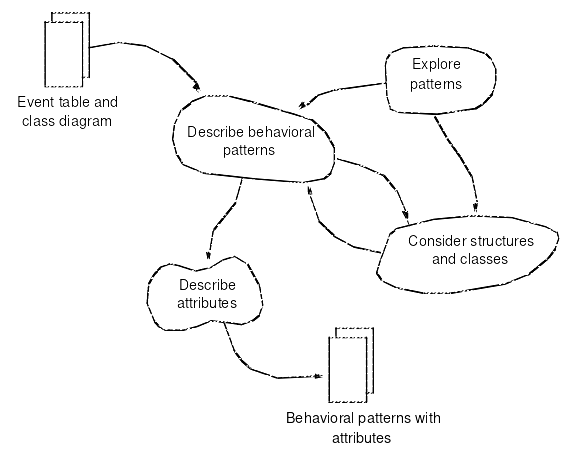
\includegraphics[width=0.65\textwidth]{figures/behaviouractivities.png}
\end{figure}

\subsection{Key concepts}
\subsubsection{Event Traces}
Event trace: A sequence of events involving a specific object. A customer object in figure \ref{fig:behaviouralpattern} might have following event trace: account opened - amount deposited - amount withdrawn - amount deposited - account closed. 

\subsubsection{Behavioural pattern}
For practical reasons, groups of objects are described instead of describing behaviour of every object. For the same reasons, the behaviour of every object is not described, instead we describe a behavioural pattern for object classes. \newline \textbf{Behavioural pattern:} A description of possible event traces for all objects in a class. 
The behavioural pattern describes behaviour common to all objects of the class. 

\begin{figure}[h]\label{fig:behaviouralpattern}
    \centering
    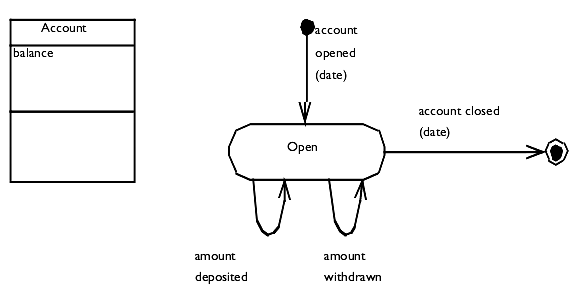
\includegraphics[width=0.6\textwidth]{figures/behaviouralpattern.png}
\end{figure}

\subsubsection{Describe behavioural patterns}
Make event traces for each class. For each of these classes, ask the following:

\begin{itemize}
    \item Which event(s) cause the creation of a problem-domain object? \newline These events are grouped as selections that can cause the creation of an object.
    \item Which event(s) cause the disappearance of a problem-domain object? \newline These events are grouped as selections that can cause the death of an object.
\end{itemize}

\noindent Typical event traces can be found with the following questions:
\begin{itemize}
    \item Which events occur together in a sequence?
    \item Are there any alternative events?
    \item Can a given event occur more than once?
    \item Is the overall form structured or unstructured?
\end{itemize}


\subsubsection{Control structures}

A behavioural patterns orders individual events in time using control structures:

\begin{itemize}
    \item \textit{Sequence:} Events in a set occur one by one. Denoted using "+"
    \item \textit{Selection:} Exactly one out of a set of events occurs. Denoted using "l"
    \item \textit{Iteration:} An event occurs zero or more times. Denoted using "*"
\end{itemize}

A behavioural pattern with these can be described with a regular expression. For example: account opened + (amount deposited | amount withdrawn)* + account closed.

A statechart diagram has the same expressive capability as the regular expression, and these are drawn as such:

\begin{figure}[H]
    \centering
    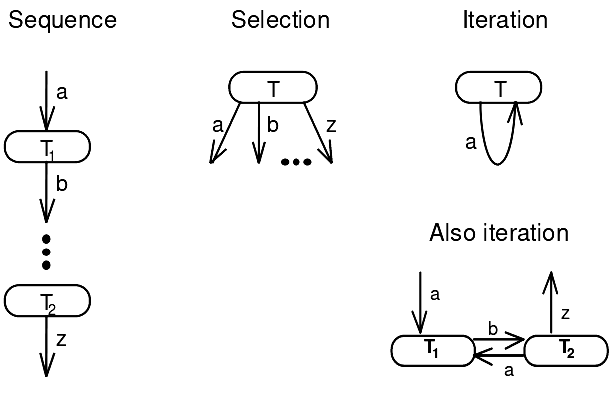
\includegraphics[width=.5\textwidth]{figures/behaviouralcontrol.png}
\end{figure}

\subsection{Modelling techniques}
\subsubsection{From event traces to behavioural patterns}
\begin{figure}[H]
    \centering
    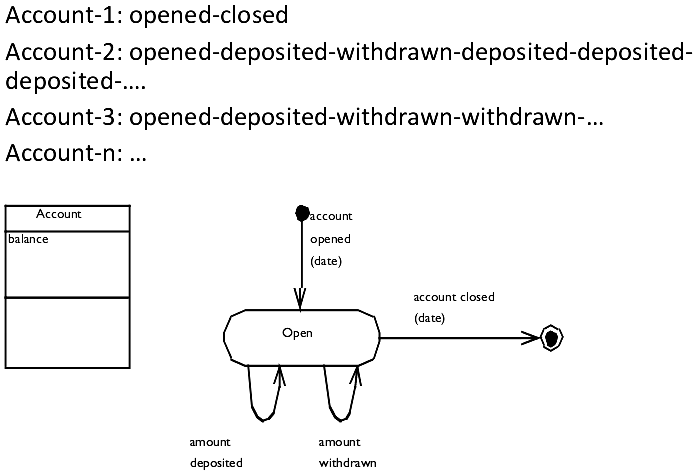
\includegraphics[width=.75\textwidth]{figures/eventtracetobehaviouralpattern.png}
\end{figure}

It's clear that all event traces can be represented through the actions of the behavioural pattern. 

\subsubsection{Conditions in statechart diagrams}
Typically the transition in a statechart diagram occurs as a result of problem-domain events. In special cases you may want to supplement with another form of transition - one that occurs when a stated condition is true. 

The requirement is stated in the square brackets in the figure. This conditional transition is useful both with administrative and technical systems.

\begin{figure}[H]
    \centering
    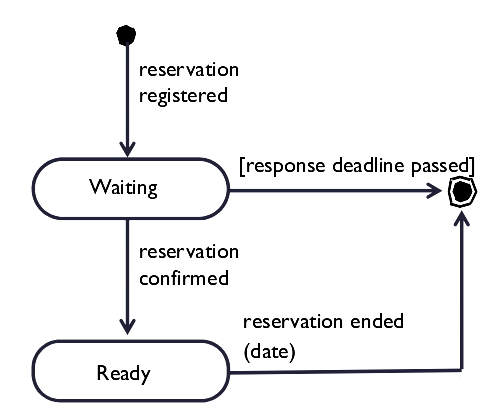
\includegraphics[width=.4\textwidth]{figures/conditionalstatechart.png}
\end{figure}

\subsubsection{Common events}
It's useful to create behavioural patterns for common events, as these are naturally the most abundant in the system to be designed.

\subsubsection{Consider structures}
Aggregation and association:
\begin{itemize}
    \item If two or more objects have common events, consider adding an aggregation or association structure between them.
    \item If two classes are related by an aggregation or association structure, at least one common event should be considered.
\end{itemize}
\noindent Generalisation:
\begin{itemize}
    \item If the same event is tied to two classes, consider whether one class is a generalisation of the other.
\end{itemize}

\subsubsection{Hierarchical states}
Consider using this pattern to simplify modelling.

\begin{figure}[H]
    \centering
    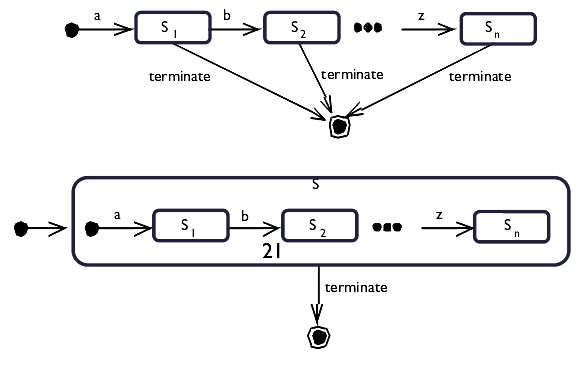
\includegraphics[width=.65\textwidth]{figures/hierarchicalstate.png}
\end{figure}

\subsubsection{Describe attributes}
The following questions can be asked to describe attributes. Class attributes:
\begin{itemize}
    \item What are the general characteristics of the class?
    \item What basic data must be captured about the objects from this class?
    \item What results from an event trace must be captured?
\end{itemize}

\noindent Event attributes:
\begin{itemize}
    \item What time did the event occur?
    \item Which amount did it concern?
\end{itemize}


\subsection{Summary}
\begin{figure}[H]
    \centering
    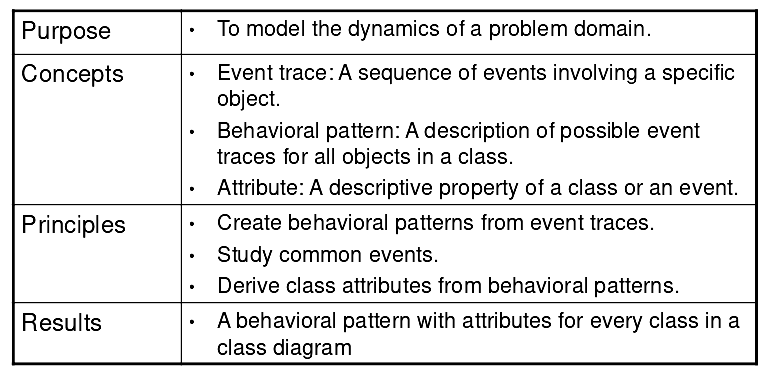
\includegraphics[width=.7\textwidth]{figures/behavioursummary.png}
\end{figure}

\section{Example on streaming}\label{behaviour:streamingservice}
Recall the FACTOR-description and class diagram from section \ref{structure:streamingservice} on a streaming service. Following are three statechart diagrams for Customer, watched, and Movie:

\begin{figure}[H]
    \centering
    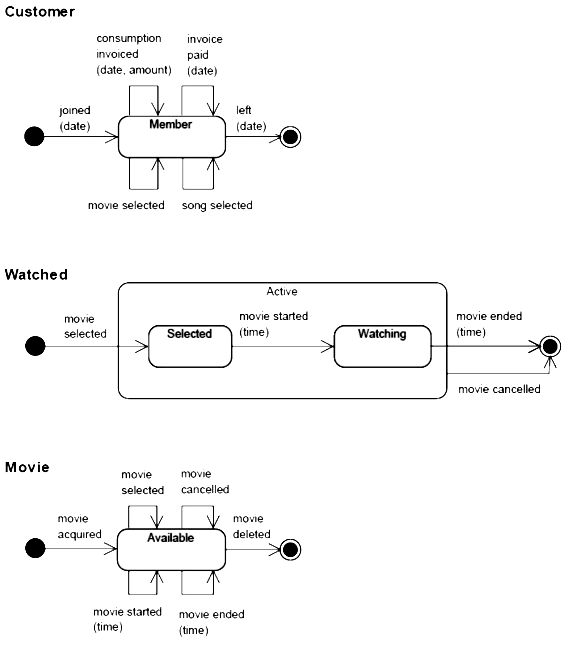
\includegraphics[width=.6\textwidth]{figures/statechartstreaming.png}
\end{figure}

\section{Explore patterns}
We'll focus on three basic behaviour patterns. These can be used to improve an outline or contribute to a completely new idea for part of the problem-domain model.

\subsection{Stepwise relation pattern}
\begin{figure}[H]
    \centering
    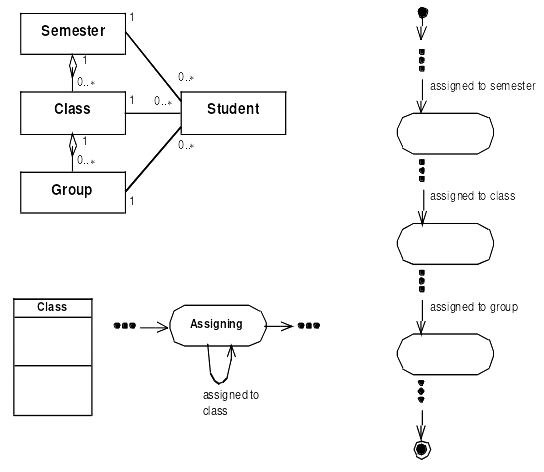
\includegraphics[width=.6\textwidth]{figures/stepwiserelation.png}
\end{figure}

This pattern is used when the elements of a hierarchy  resembles a stepwise or sequential manner. The figure shows a situation where students are first assigned a semester, then a class, and lastly a group. The group is an element of a class, the class is an element of a semester.

\subsection{Stepwise role pattern}
\begin{figure}[H]
    \centering
    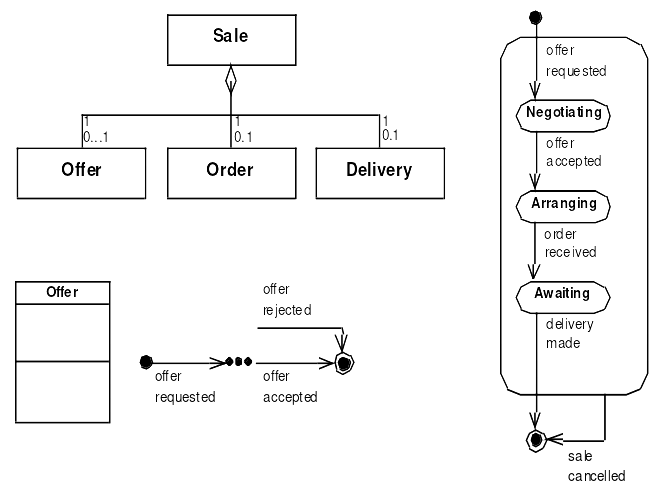
\includegraphics[width=.6\textwidth]{figures/stepwiserole.png}
\end{figure}

This pattern is used to describe interaction between several objects over time, but more-so on the horizontal dimension in a class diagram than the vertical dimension.
The figure shows a sale modelled as consisting of an offer, an order, and a delivery. The statechart diagrams show how these objects interact and gets created. E.g. an offer is created when it is requested, and terminates when the offer is accepted or rejected. The two other subobjects behave similarly.
A sale can be terminated at any time in the course of its life, as shown by \texttt{sale cancelled}.

Note that this pattern is simple when the order is sequential. As soon as the parts become interwoven and mutually dependent the complexity of the diagram increases rapidly.
\subsection{Composite pattern}
\begin{figure}[H]
    \centering
    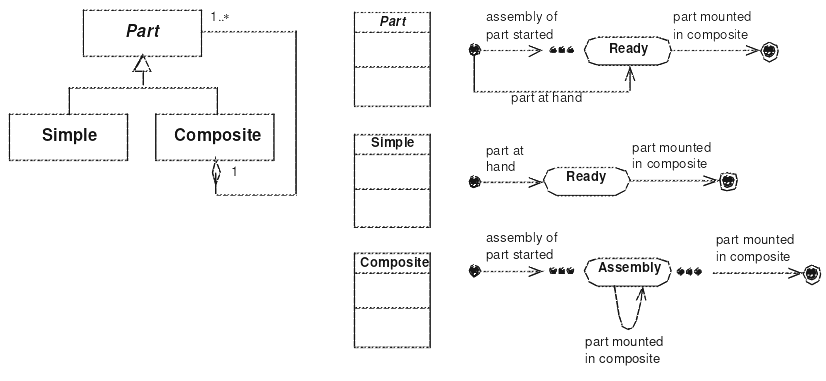
\includegraphics[width=.8\textwidth]{figures/compositepattern.png}
\end{figure}

This pattern offers a way to describe the creation and destruction of a hierarchy using a detailed structure that is unknown at model-development time. 
The figure shows an example, where \texttt{Part} is an abstract class, and \texttt{Simple} and \texttt{Composite} are specialisations. A composite part aggregates several parts, where each part is one of the two specialisations.

The figure also shows the behavioural patterns for the tree classes. A parts statechart diagram imposes limits on specialisations. A simple part is immediately ready, as it does not need assembly. If this simple part is mounted in a enclosing composite its separate life ends and it continues to live on only as an integrated part of a composite. Likewise, if the composite is mounted, with all it subparts, on another composite, its life is terminated and it continues on as a part of a new composite.

The key point in this pattern is that the top-level behaviour requires some behaviour from the level beneath it, which in turn requires behaviour from the level beneath it, and so on. This ends up being a recursive description. 

\section{Conceptually; class, event, or attribute?}
We have some information from the problem domain, e.g., a customer buys a chair for 100 DKK. How can this be modelled?

\begin{itemize}
    \item \textbf{Attribute:} In the Customer class we introduce an attribute \texttt{bought} which is increased by the amount that the customer has bought for.
    \item \textbf{Event:} For the Customer class we introduce a \texttt{bought} event with the price of the chair as an attribute. This allows us to produce a list of the amounts the user has purchased for.
    \item \textbf{Class/Object:} We introduce a \texttt{Bought} class that is aggregated by the Customer class, it aggregates an object of the Product class and has some events. This allows us to model events for and behavioural structure on \texttt{Bought} objects.
\end{itemize}

\section{Principles}
\subsection{Create behavioural patterns from event traces}
The problem-domain dynamics are described by behavioural patterns for each class in the model. The behavioural pattern describes legal event traces and thereby determines the order of events for each object in the class.

\subsection{Study common events}
Common events point out important, dynamic relations in the model. common events can cause reconsideration of the choice of classes and their structural relations.

\subsection{Derive class attributes from behavioural patterns}
The attributes necessary for capturing relevant data about objects and events are derived from the class definition and the behavioural pattern.

\section{Challenges in this activity}
\begin{itemize}
    \item Start with event traces for the simple classes
    \item Describe behavioural patterns from the event traces
    \item Continue with the more complex classes
    \item If the behavioural pattern becomes too complicated, consider using the stepwise role or stepwise relation pattern - \textit{this introduces new classes}
    \item Make sure there are behavioural patterns that control sequence and some that don't (structured/unstructured)
    \item Add attributes to classes and events
    \item Check the behavioural patterns against the class diagram
\end{itemize}
\chapter{Lecture five: Usage}

\section{Application Domain Analysis}
Application-domain analysis focuses on a question: How will the target system be used? The purpose is to define requirements for the system's functions and interfaces.

\subsection{Result}
A complete list of the system's overall usage requirements. This includes actors and use cases, user interfaces and functions. 

\subsection{Key concepts}
\textbf{Application domain:} The organisation that administrates, monitors, or controls a problem domain. 

\subsubsection{New concepts}
New concepts in the application domain analysis includes:
\begin{itemize}
    \item Actors (users and other systems)
    \item Use cases
    \item Functions
    \item Interfaces
\end{itemize}

\subsection{Using the model of the problem domain}
Stage's infamous penis-model-drawing is included here.
\textbf{Model:} A description of classes, objects, structures, and behaviour in a problem domain. Provides an updated representation of the state in the problem domain. 

In analysis, we describe the problem domain by an object-oriented model. We also describe how the model is used in the application by the actors.

\subsection{Activities}
This is the finding of usage, functions, and interfaces. Defining requirements is an iterative activity alternating between usage, functions and interfaces. These three will be discussed in chapters 6-8.

\begin{table}[]
\centering
\begin{tabular}{lll}
\hline
\multicolumn{1}{|l}{\textit{\textbf{Activity}}} & \textit{\textbf{Content}} & \multicolumn{1}{l|}{\textit{\textbf{Concepts}}} \\ \hline
Usage & \begin{tabular}[c]{@{}l@{}}How does the system interact \\ with people and \\ systems in the context?\end{tabular} & Use case and actor \\
Functions & \begin{tabular}[c]{@{}l@{}}What are the sytem's\\ information processing \\ capabilities?\end{tabular} & Function \\
Interfaces & \begin{tabular}[c]{@{}l@{}}What are the target system's \\ interface requirements\end{tabular} & \begin{tabular}[c]{@{}l@{}}Interface, user interface,\\ and system interface\end{tabular} \\ \hline
\end{tabular}
\end{table}

\subsection{Stable versus transient properties}
The different properties in the system has different levels of stability. When the model is changed, all the functions and interfaces must change also. However, the functions can be changed, without changing the model. Interfaces can also be changed, without changing the functions or the model. The model is therefore more stable. In practice, the system model changes more rarely than the function or interface requirements.

\begin{figure}[H]
    \centering
    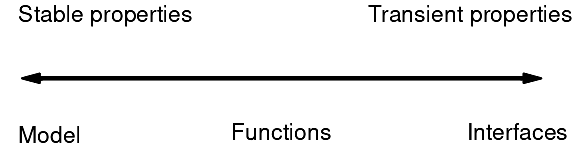
\includegraphics[width=.6\textwidth]{figures/properties.png}
\end{figure}

\subsubsection{Classical vs modern bank}
The model is the same. The basic functions are the some, withdraw and deposit, but new ones are added, e.g. MobilePay. Interfaces are however completely changed.
\begin{table}[h]
\centering
\begin{tabular}{|l|l|l|}
\hline
 & Classical bank & Modern bank \\ \hline
Model & Identical & Identical \\ \hline
Function & Withdraw and deposit & Also with/deposit, however also transactions \\ \hline
User interface & Different & Different \\ \hline
\end{tabular}
\end{table}

\subsection{Summary}
\begin{figure}[H]
    \centering
    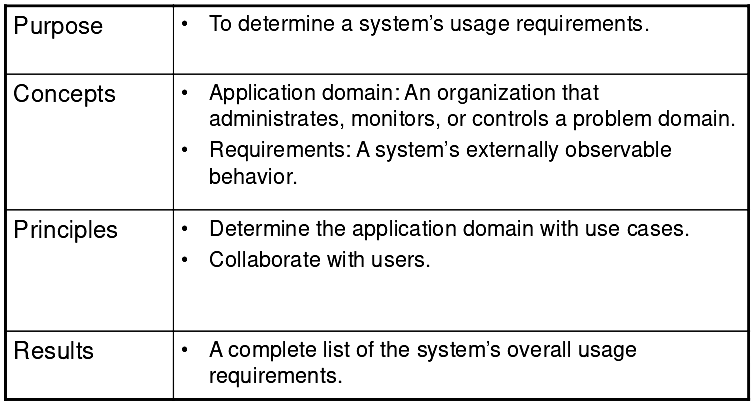
\includegraphics[width=.6\textwidth]{figures/apdomainsummary.png}
\end{figure}

\section{Usage}
\subsection{Results}
Descriptions of all \textbf{use cases}, \textbf{actors}, and an \textbf{actor table}.
\begin{figure}[H]
    \centering
    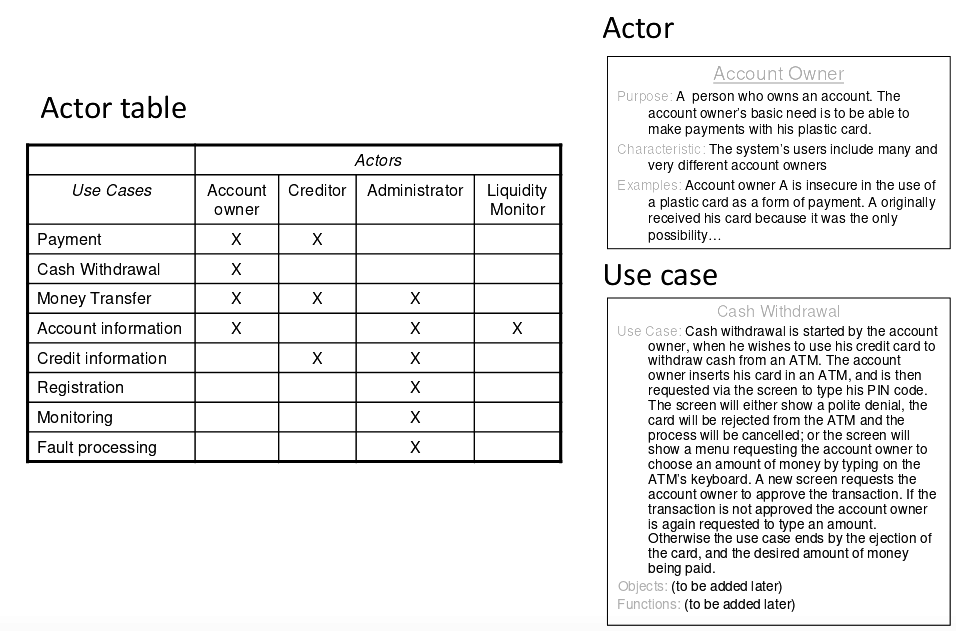
\includegraphics[width=\textwidth]{figures/usageresults.png}
\end{figure}

\subsection{Start out from work tasks}
What tasks exist in the application domain? How is the division of labour? How are the different tasks delimited?

\noindent Describe the tasks:

\begin{itemize}
    \item Name and content
    \item Purpose
    \item How is it assigned?
    \item Who performs it?
    \item Relationship to other tasks
    \item Result
\end{itemize}

For example, an administration system's work tasks:

\begin{itemize}
    \item Establish new conference
    \item Detailed planning of conference
    \item Administration of participants
    \item Registration of person
    \item Administration of articles
    \item Information to the committees
    \item Information to participants, authors, and reviewers
\end{itemize}

\subsection{Key concepts}
\subsubsection{Actor}
Identify actors:
\begin{itemize}
    \item Determine the distribution of roles of the work tasks related to the system
    \item Consider human actors
    \item Consider other systems as actors
\end{itemize}

\noindent Lastly, describe these actors in terms of \textbf{purpose, characteristics, and examples}. E.g. an account owner in a bank could be described as the following:

\begin{itemize}
    \item[] \textbf{Purpose:} A person who owns an account. The account owner's basic need is to be able to make payments with his plastic card.
    \item[] \textbf{Characteristic:} The system's users include many and very different account owners.
    \item[] \textbf{Example A:} Account owner A is insecure in the use of a plastic card as a form of payment. A originally received his card because it was the only possibility for getting an ID card for his checks. A only withdraws money from the ATM in emergency situations.
    \item[] \textbf{Example B:} Account owner B is technologically curious and uses the system often, optimally, and to the limit of its abilities. B has never had major problems in understanding the possibilities of the system, and B also examines the possibilities that are not obviously available.
\end{itemize}


\subsubsection{Use cases}
Identify use cases where the system is used to carry out part of a work task. Describe use cases; as text or as a state-chart diagram, or an actor-table as seen on page 123.


\noindent A \textbf{use case} based on cash withdrawal could be written like the following:

\begin{itemize}
    \item[] \textbf{Use case:} Cash withdrawal is started by the account owner, when he wishes to use his credit card to withdraw cash from an ATM. The account owner inserts his card in an ATM, and is the requested via the screen to type his PIN code. The screen will either show a polite decline, the card will be rejected from the ATM and the process will be cancelled, or the screen will show a menu requesting the account owner to choose an amount of money by typing on the ATM's keyboard. A new screen requests the account owner to approve the transaction. If the transaction is not approved the account owner is again requested to type an amount. Otherwise the use case ends by the ejection of the card, and the desired amount of money being paid.
    \item[] \textbf{Objects:} \textit{to be added later}
    \item[] \textbf{Functions:} \textit{to be added later}
\end{itemize}

It could also be drawn using behavioural patterns, like the following figure shows:

\begin{figure}[H]
    \centering
    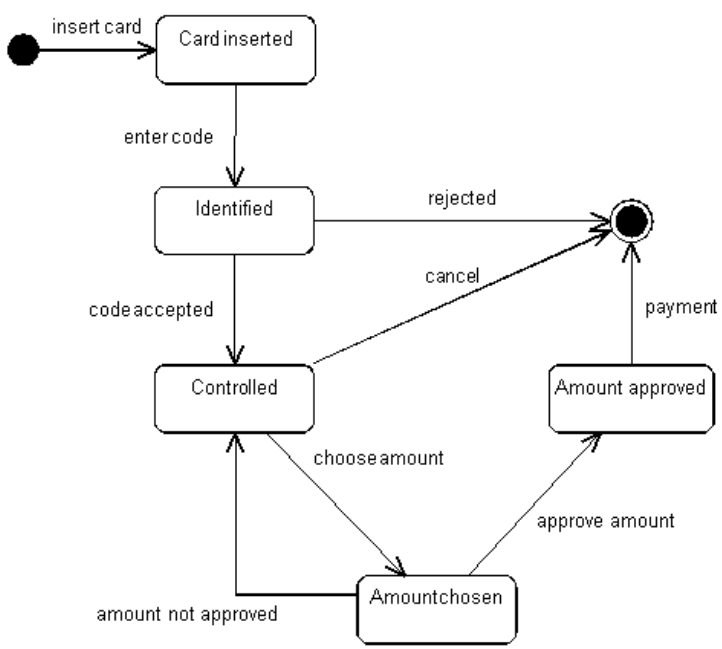
\includegraphics[width=.7\textwidth]{figures/usecasechart.png}
\end{figure}

Note that state-chart diagrams er easy and concise to discuss with peers, but users will only understand a written description of the use case.

\subsection{Activities}
Starting from a a system definition, find actors and use-cases, then both evaluate systematically and explore patterns, which lastly lead to use cases and actors.

\subsection{Evaluate systematically}
The aim is not to get a ton of details, it's to get an idea of the users and what they're doing. Do a systematic review:

\begin{itemize}
    \item Use cases should be simple and constitute a coherent whole. 
    \item The description of actors and use cases should provide understanding and overview. 
    \item Use cases should be described in enough detail to enable identification of functions and interface elements.
\end{itemize}

E.g., what could be functions and interface elements for cash-withdrawal? Also experiment with prototypes, a use case is best evaluated through planned prototype experiments.

\subsection{Summary}
\begin{figure}[H]
    \centering
    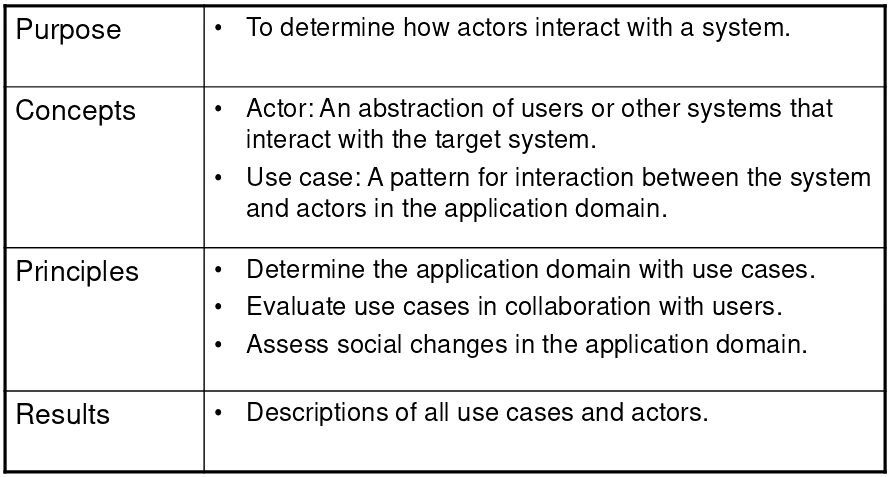
\includegraphics[width=.7\textwidth]{figures/usagesummary.png}
\end{figure}

\section{Example with a streaming service}
Recall previous class diagrams, behavioural patterns, and statechart diagrams, as seen in section \ref{behaviour:streamingservice}. An actor table for the streaming service follows:

\textit{missing from slides and therefore also from notes}

\section{Explore patterns}
\subsection{Procedural pattern}
\begin{figure}[H]
    \centering
    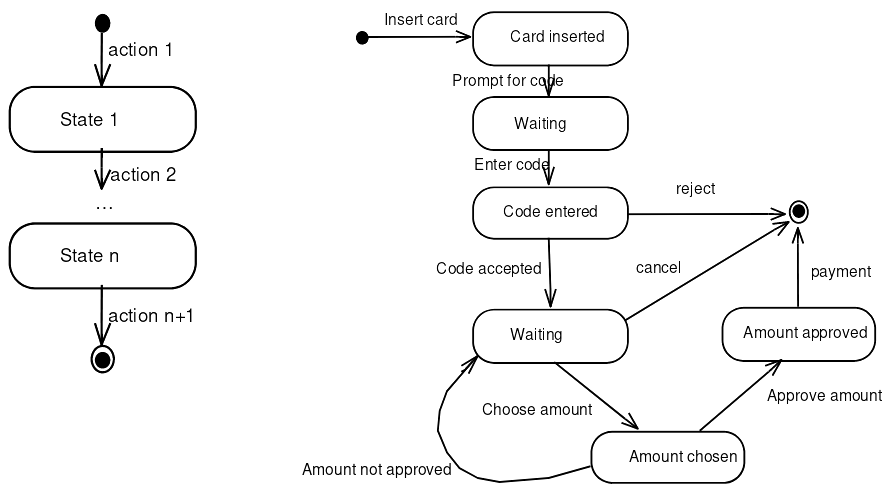
\includegraphics[width=.8\textwidth]{figures/proceduralpattern.png}
\end{figure}

Some cases dictate that certain rules are observed. In cash withdrawal for example, the actor's access rights must be established first, and there must be an extra confirmation of the withdrawal amount. This allows little variation in the actual dialogue. The use case must follow a strict procedure.

The procedural use-case pattern is the general solution to ensuring that many rules are observed. As the figure shows, the patterns basic structure is a sequence with minor variations in terms of selections or iterations. The selections and iterations can be described as nested inside the upper level states.

\subsection{Material pattern}
\begin{figure}[H]
    \centering
    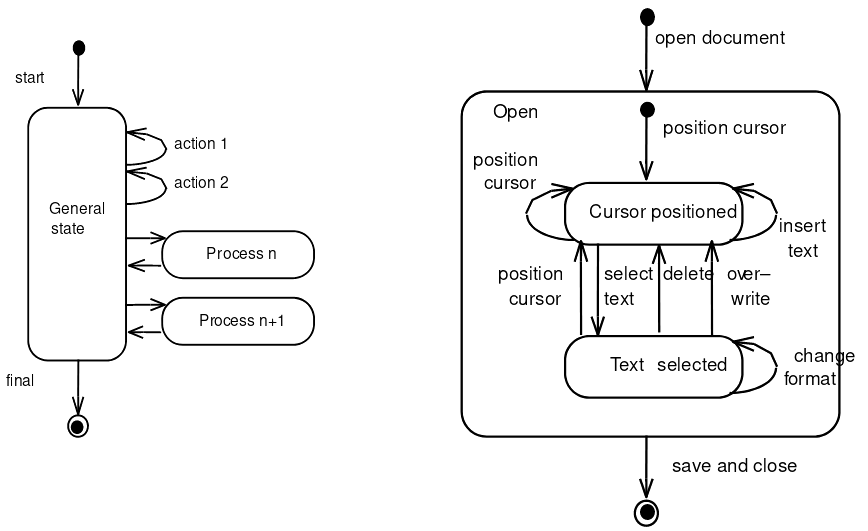
\includegraphics[width=.7\textwidth]{figures/materialpattern.png}
\end{figure}

Consider a text-editing processor. The general use case might look like what's shown in the figure; it is characterised by very little sequence and the actor can do almost anything in any order. The only restriction comes from the two modes; "cursor positioned" and "text selected", which the actor must be in to perform certain actions.

The material use case is good for situations in which there are no business-rules governing the usage. The pattern is a use-case with few general states, in which most actions can be performed. We call this the "material" use case as it resembles an artisan's material process; any tool may be used in any order.

\section{Appreciate the difference; actors and classes}
\begin{figure}[H]
    \centering
    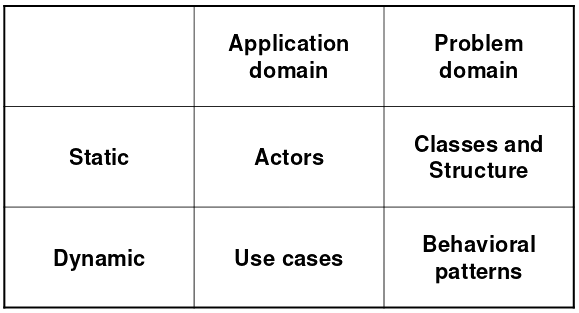
\includegraphics[width=.5\textwidth]{figures/actorvsclasses.png}
\end{figure}

\section{Principles}
\subsection{Determine the application domain with use cases}
Use cases help to focus your analysis on relevant parts of the application domain and provide descriptions at a relevant and homogeneous abstraction level. The use-case activity is an important step toward identifying requirements for the system's functions and interfaces.

\subsection{Evaluate use cases in collaboration with users}
Experiments with prototypes are well suited to use-case evaluation and can provide inspiration for new use cases.

\subsection{Assess social changes in the application domain}
Developing a new system is an opportunity to critically rethink the work organisation in the application domain. The goal is to avoid work-related problems and unnecessary human adjustments.
\chapter{Lecture six: OOA\&D in Practice}

\section{Software requirements}
\subsection{Unclear requirements}
There are many examples of problems with requirements. Unclear requirements have been denoted as the main source of problems in system development projects.

E.g: Amanda; the IT-system for Arbejdsformidlingen ended up costing 650+ million DKK, originally budgetted for 214 million DKK. It did not fit the work of the employees; for example, they had to go through 40-50 screens to register a single person as unemployed. The time spent per registration went from 10-20 minutes to one hour.

Examples of similar situations and causes of these:

\begin{itemize}
    \item Sundhed.dk; the information is flawed, it had been dropped, and rebudgeted multiple times. Few citizens know of this system.
    \item Rejsekort; didn't work well initially, you can't top up the card immediately online.
\end{itemize}

\subsection{Empirical study of practice}
The solution works as intended but doesn't match the context - which is the AD and PD.

Requirements might be wrong, but the programmers implement them anyway, or vice versa.

E.g; the users are not satisfied with the product. They find it too difficult to use, unable to support certain user tasks, or the program doesn't cooperate properly with existing, surrounding software.

\subsection{Experiment}
Take an existing product, find flaws and the solutions to them, then implement techniques to avoid those, and try the best of them in new projects.

Find cost-effective ways to avoid defects in products.

This was tried out by Brüel \& Kjaer\footnote{Sound and vibration specialists}, whom manufacture professional equipment for sound and vibration measurement, and more than half of the product developers are software-developers. They develop products in accordance with the \textbf{waterfall-model} where phases can only overlap to some extent. They talk about phases such as requirements specification, design, programming, module test, integration test. 

From integration-tests, they routinely record all defects detected by programmers, in-house product testers, marketing, and customers.

\subsection{Examples of requirements}
A good way of assuring the measurement quality is to examine the measured spectra. This allow the experienced user to determine the quality of the measurement. For example:

\begin{itemize}
    \item R-25: During the measurements the application must show the latest measured spectrum.
    \item ...
    \item R-35: The application must be able to display all results, even if some of the points have not been measured.
\end{itemize}

The requirement specification that resulted from this experiment is a total of 20 pages with 107 requirements. 

\subsection{Analysis of defect reports}
Around 800 defect reports collected a few months after product release, 107 reports analysed in detail. Major sources of defects:
\begin{itemize}
    \item \textbf{Missing requirements}; i.e. requirements that had not been written down in the spec and were not otherwise transferred to developers (45 cases): ignored or forgotten (21 of the 45 or not recognised although they had been present in the domain all the time (24 of the 45)
    \item \textbf{Mistaken tacit requirements}; i.e., the developer somehow knew about the demand, but made a wrong solution (24 cases): made a wrong guess (nine of the 24) or couldn't resolve apparently conflicting or inconsistent demands (15 of the 24).
    \item \textbf{Mistaken specs}; i.e., written requirements that were implemented incorrectly (14 cases): a simple mistake (four of the 14), a misunderstanding of the spec (two of the 14), inconsistent requirements (two of the 14) or broad requirements that were not fully implemented everywhere, e.g. that \textit{'the interface shall follow the Windows style guide'} (six of the 14).
    \item \textbf{Defects relation to external software}; misunderstood how external software worked or the external software didn't work correctly, or didn't fulfil expectations
\end{itemize}

They also classified each defect according to the quality factor (McCall) that was impaired, e.g., functionality, usability, or maintainability. Almost 70\% of the defects were related to usability (ease of understanding and use).

\subsection{Defects and potential techniques}
Defects in existing products:

\begin{itemize}
    \item 60\% of the defects related to unstated demands (tacit requirements)
    \item Almost 70\% of the defects had to do with ease of understanding or ease of use (usability)
    \item Most related to the user interface and misunderstood interfaces to third-party software
\end{itemize}

\noindent Potential techniques:

\begin{itemize}
    \item Identified 44 techniques from literature or practice
    \item For each defect they identified the techniques that might find or prevent the defect - and with what probability
    \item About ten techniques were worth considering in a project of this kind
\end{itemize}
\subsection{Measured effect in new project}
The new project; the user tasks were studied directly and the user interface was designed and usability tested before any part of it was programmed. Obstacles:
\begin{itemize}
    \item Some top techniques were useful in one kind of project, but much less important in other projects
    \item The organisational surrounding may block the use of some techniques
    \item Developers have difficulties using many new techniques at the same time
    \item Unforeseen events, such as a new project manager, can overturn earlier decisions to use a certain technique
\end{itemize}

\noindent The new project experienced:
\begin{itemize}
    \item The number of usability problems per screen was reduced by around 70\%, expected around 18\% reduction
    \item The project was the first one of theirs to be completed on time and without stress
    \item The product sound twice as many units as comparable products and at twice the unit price
\end{itemize}

\section{Construction and iteration}
\subsection{Waterfall-model}
\begin{figure}[H]
    \centering
    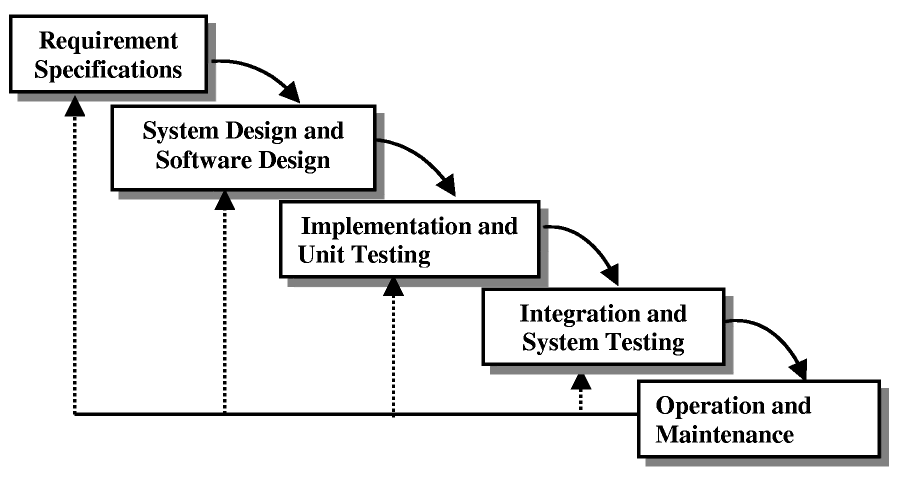
\includegraphics[width=.6\textwidth]{figures/waterfallmodel.png}
\end{figure}

A number of phases exist; requirements, design, implementation, verification, maintenance. Each phase has a clear purpose. It is necessary to be able to define the problem very precisely and in detail. A number of challenges exist:

\begin{itemize}
    \item Based only on specifications but they are difficult to produce and understand
    \item Difficult to get the users to describe their work
    \item Non-technical aspects are difficult to specify
    \item Requirements are changing over time
    \item Works only when we know exactly what we want and we are able to describe it precisely and unambiguously
    \item Feedback loops become necessary
    \item Many negative effects of the systems developed
\end{itemize}

\subsection{Iterative-model}
\begin{figure}[H]
    \centering
    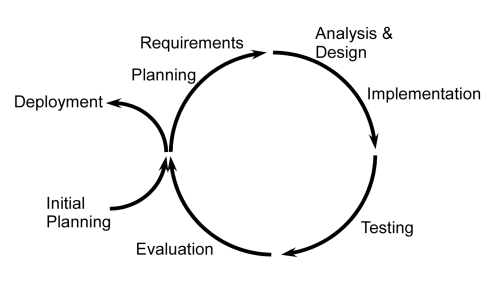
\includegraphics[width=.4\textwidth]{figures/iterativemodel.png}
\end{figure}
A model of steps that can be iterated a number of times.

\begin{itemize}
    \item Evolution with prototypes
    \item No set of clear requirements to depart from
    \item The understanding of the problem is changing during development
    \item Development through a series of cycles
    \item The requirements and the system are improved in each iteration
\end{itemize}

\subsection{Example one}
The B\&K systems were developed with a waterfall model and it involved a number of phases from requirements to release. The new project involved prototype development and some evaluation in the requirements phase, therefore some iteration was present.

\subsection{Example two}
Visualisation of blood tests results for diagnosing\footnote{Adam Viggo Glistrup and Dennis Dalgaard (2016) UI Prototypes ‐ Identification of software requirements in a highly complex domain. Master thesis, Aalborg University, Department of Computer Science.}.

Impossible for developers to learn enough about the diagnosis process to enable them to produce a prototype. The preference of doctors is an important point as well. Boundary object; physical object with different representation, drawings, illustrations, and more. Used boundary objects to facilitate discussion with the medical doctors and illustrate options.

\section{Contingency theory}
How do you intelligently choose between waterfall- and iterative-method? The relevance of these categories of methods can be determined from contingency factors. Analyse uncertainty in terms of the following four factors:

\begin{itemize}
    \item the organisational and technical context of the system
    \item the future computer system
    \item the experience and skills of the users
    \item the experience and skills of the system developers
\end{itemize}

Selection of approach; if uncertainty is low, base requirements determination of an informal approach or on analysis of existing systems, or if uncertainty is high, use specifications or prototypes. 

Furthermore; there's a distinction between complexity and uncertainty.

Uncertainty is; the degree of structuredness that characterises the users' work, the degree of understanding the users have about their work, and the degree of experience and training of the system developers.

Complexity is; the project size, number of users, volume of new information, and complexity of new information.

\begin{figure}[H]
    \centering
    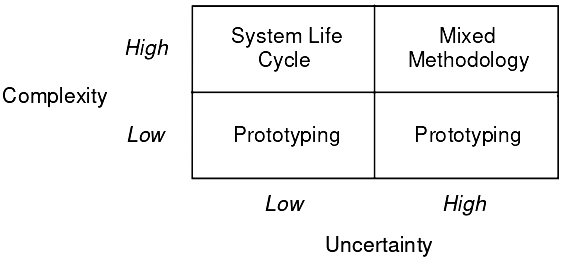
\includegraphics[width=.5\textwidth]{figures/complexityuncertaintymodel.png}
\end{figure}

\subsection{Principle of limited reduction}
Contingencies should be analysed dynamically throughout a development project. The principle of limited reduction: 

\begin{figure}[H]
    \centering
    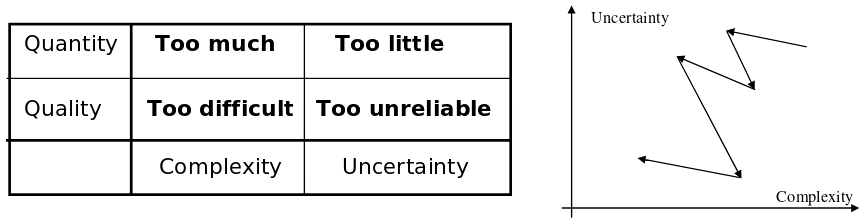
\includegraphics[width=.5\textwidth]{figures/limitedreduction.png}
\end{figure}

\begin{itemize}
    \item Relying on an analytical mode of operation \textit{to reduce complexity} introduces new sources of uncertainty requiring experimental countermeasures.
    \item Relying on an experimental mode of operation to \textit{reduce uncertainty} introduces new sources of complexity requiring analytically countermeasures.
\end{itemize}

\section{Strategy with \ad}

Top-down strategy means doing each task sequentially, almost waterfall-ish but in one stretch, executing quality assurance periodically. Similarly, \textit{use-case driven}, architecture-centric, and incremental methods iterate each prototype incrementally based on some requirement, that being user-stories, etc.

\subsection{Activities}
From existing documentation, the task is characterised, difficulties are evaluated, a strategy is formulated, which leads to an \textbf{analysis and design strategy}, which guides the object-oriented analysis and design (\ad).

\subsection{Characterise the task}
Using a checklist, asking questions on the basic characteristics of the task and the actors interacting with it, both during development and eventual use. Whichever part of the checklist that has the most uncertainty should be the focus of the strategy. Tailor the strategy to resolve these difficulties first. 

\begin{figure}[H]
    \centering
    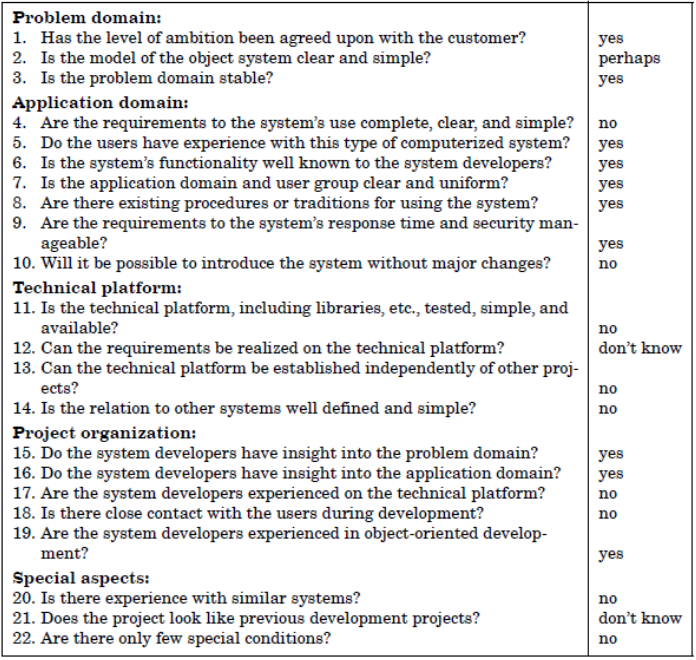
\includegraphics[width=.7\textwidth]{figures/checklist.png}
\end{figure}

\subsection{Evaluate difficulties}
Using the checklist, grade each activity on difficulty as $0$ for yes, $1$ for perhaps, and $2$ for no or unknown. This gives you an overview of the most difficult activities in the \ad-method. Then tailor the strategy to resolve the most significant difficulties first.
\begin{figure}[H]
    \centering
    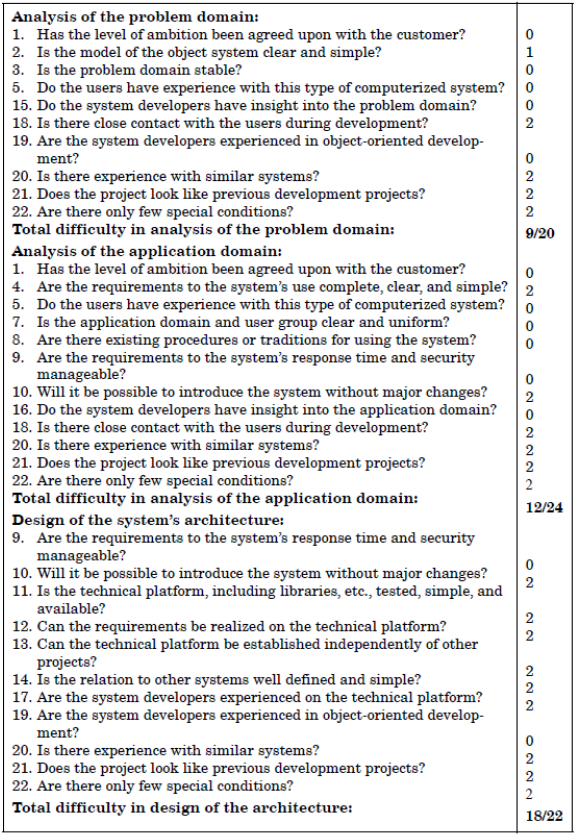
\includegraphics[width=.7\textwidth]{figures/checklistevaluatediff.png}
\end{figure}

\subsection{Summary}
\begin{figure}[H]
    \centering
    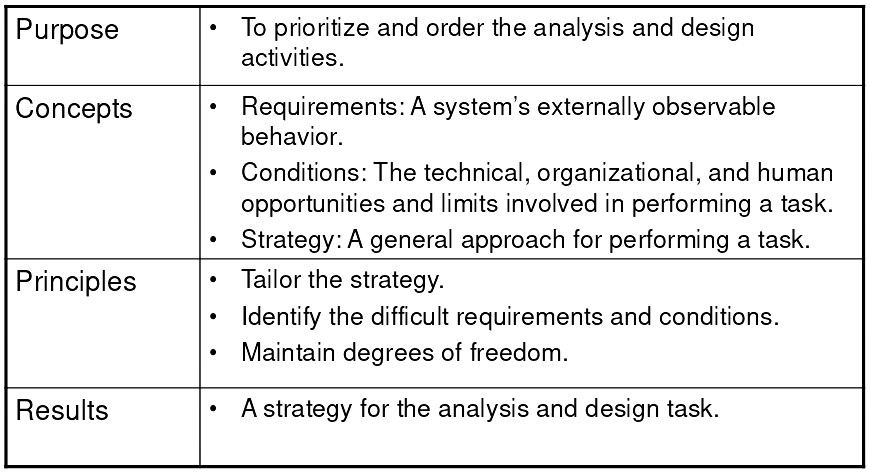
\includegraphics[width=.7\textwidth]{figures/strategysummary.png}
\end{figure}

\section{Principles}
\subsection{Tailor the strategy}
To efficiently use development resources to mange difficulties in a software project, a strategy must be tailored to the situation.

\subsection{Identify the difficult requirements and conditions}
The big project challenges and problems stem from disparity between requirements and realities. It is important that the development strategy identifies critical areas that require special effort and attention.

\subsection{Maintain degrees of freedom}
Unexpected problems will appear during analysis and design. The strategy should ensure that degrees of freedom are maintained for a possible redesign of system parts later in the process.


\chapter{Lecture seven: Functions}
\section{Difficulties}

\subsection{Final state for an object}
What happens when an object gets to the final state? Does it die, disappear, or what? \newline \textbf{In analysis:}

\begin{itemize}
    \item The object can no longer perform or suffer events
    \item The state of the object can still be read by a function
\end{itemize}

E.g. a bank account object must exist after we have closed it, so we can read it; e.g. to produce information to the customer and tax authorities at the end of the year. \newline \textbf{In design:}

\begin{itemize}
    \item Decide for how long we'd want to keep objects who are in their final states
    \item E.g. there are laws that define how long a bank account object that is in it's final state (closed) must be kept
\end{itemize}

\subsection{Iteration in state chart diagrams} 

\begin{itemize}
    \item when should we put iteration in the event table and when is it not an iterative event?
    \item How should we describe iteration in the state chart diagram? Should it be through another state and back, or through a loop-arrow?
\end{itemize}

\begin{figure}[H]
    \centering
    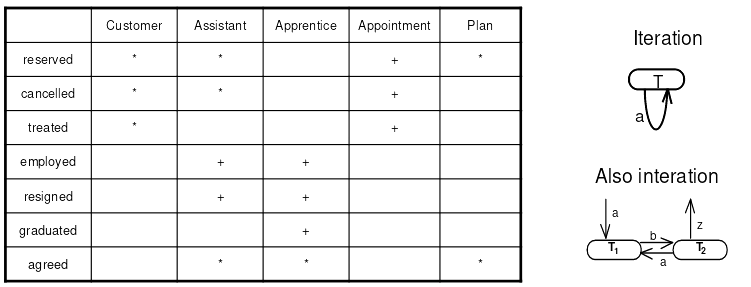
\includegraphics[width=.8\textwidth]{figures/difficultiesiteration.png}
\end{figure}
 

\subsection{Item-Descriptor pattern and the behaviour of the classes} why and when should we use it; and how to we create behavioural patterns for the item and descriptor classes? Generally, it's the distinction between the description/template of the thing, and the instance of the thing.

\begin{figure}[H]
    \centering
    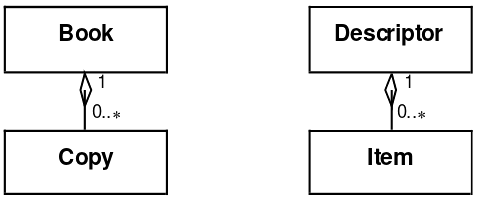
\includegraphics[width=.5\textwidth]{figures/difficultiesitemdescriptor.png}
\end{figure}

\textbf{Events:}
\begin{itemize}
    \item Descriptor: book created, book deleted
    \item Item: copy borrowed, copy returned
    \item Common events: copy bought, copy destroyed
\end{itemize}

\subsection{Actor}
An actor is a user, person, or system interacting with the system that is being developed. Example:

\begin{figure}[H]
    \centering
    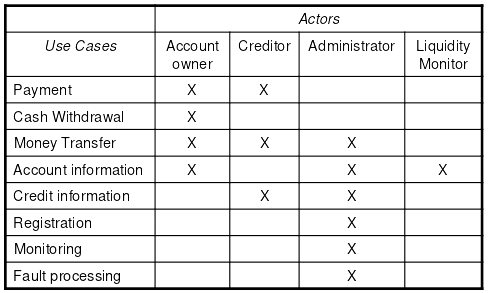
\includegraphics[width=.5\textwidth]{figures/difficultiesactor.png}
\end{figure}

\section{The function activity}
\subsection{Results}
\textbf{Primarily;} a complete list of functions with information of complexity and place of execution. 

\begin{figure}[H]\label{fig:primaryfunctions}
    \centering
    \includegraphics[width=.5\textwidth]{figures/primaryfunctions.png}
\end{figure}

\textbf{Secondarily;} a specification of complex functions with explicit states, and input/output. The aim of this activity is to identify the difficult-to-write functions.

\begin{figure}[H]
    \centering
    \includegraphics[width=.5\textwidth]{figures/secondaryfunctions.png}
\end{figure}

\subsection{Key concepts}

\subsubsection{Function types}

Function: a facility for making a model useful for actors. A function is activated, executed, and provides a result. Function execution can change a model component's state or create a reaction in the application or problem domains. a function is a requirement. Functions are rarely "pure", but often a combination of more than one of the four types:

\begin{itemize}
    \item \textbf{Update} functions are activated by a problem-domain event and result in a change in the model's state
    \item \textbf{Signal} functions are activated by a change in the model's state and result in a reaction in the context; this might be a display to actors in the AP, or direct intervention in the PD.
    \item \textbf{Read} functions are activated by a need for information in an actor's work task and result in the system displaying relevant parts of the model
    \item \textbf{Compute} functions are activated by a need for information in an actor's work task and consists of a computation with data from the actor or model; result is a display of the computation's result
\end{itemize}

\begin{figure}[H]
    \centering
    \includegraphics[width=.5\textwidth]{figures/functiontypes.png}
\end{figure}

\subsection{Activities}
The central point of system-functionality analysis is ending with a list of function that is complete and consistent with the use cases. The functions must be consistent with the other analysis results. in particular, functions must support the use cases, and all parts of the model should be used by some function. Only detailed descriptions should be given for the most complex and incomprehensible functions. Three activities in function analysis: Find functions, specify complex functions: and evaluate critically.
\\\textbf{Principles:}
\begin{itemize}
    \item Identify all functions
    \item Specify only complex functions
    \item Check consistency with use cases and the model
\end{itemize}

\begin{figure}[H]
    \centering
    \includegraphics[width=.7\textwidth]{figures/functionsactivities.png}
\end{figure}

\subsubsection{Find functions: Update}
Classes typically give rise to read and update functions. Events lead to requirements for update functions. Use cases give rise to all types of functions. Updating is related to events in the problem domain. For each event ask:

\begin{itemize}
    \item How is the event observed, and how is it registered? In which use cases does this happen?
    \item How should the use cases be supported by update functions?
    \item Which objects, attributes, and object structures are affected by the event, and what requirements does this impose on the update functions?
\end{itemize}

\subsubsection{Find functions: Read}
Classes typically give rise to read and update functions, Use cases give rise to all types of functions. Reading reflects a need for information in the application domain about the problem domain. \\
\textbf{Actor perspective:}
\begin{itemize}
    \item Given the work of the actors, what do the actors need to know about the state of the model? What read functions does this give rise to?
\end{itemize}
\textbf{Model perspective:}
\begin{itemize}
    \item Given the model, which objects and structures will the actors need information about? What read functions does this give rise to?
\end{itemize}

\subsubsection{Find functions: Compute}
Use cases give rise to all types of functions. Computation is used to generate further information. Take your point of departure in actors and use cases:
\begin{itemize}
    \item Which computations (not necessarily based on the model) do the actors need to have carried out?
    \item Does the computational basis come from the actors, the model, or both?
    \item Which computations form complete wholes in the use cases?
\end{itemize}

\subsubsection{Find functions: Signal}
Use cases give rise to all types of functions. Signalling is related to critical states in the model. Examine the model of the problem domain carefully:
\begin{itemize}
    \item What are the critical states for the model?
    \item What is the significance of these critical states? What are the consequences when they occur?
    \item How does a signal function register that the model has entered a critical state?
    \item What signals does each critical state give rise to? How reliable and strong do the signals have to be?
\end{itemize}


\subsubsection{Specify complex functions}
A detailed description might be needed to understand a function sufficiently and to realistically assess its complexity. In most cases this is not necessary during analysis. Basic rule dictates functions should be briefly and informally describes in a list. Only detailed description for special cases. Several methods can be used for this detailed description:

\noindent \textbf{Mathematical expression} can be used, where the relation between input data and output data is specified as $o = f(i)$
\\\textbf{Algorithm} can be described using pseudocode.
\\\textbf{Decomposition} is the further partitioning of a function in the function list, such as the one in figure \ref{fig:primaryfunctions}, showing the complete functional hierarchy directly in the list. A hierarchical function list gives a better overview than a standard list.
\begin{figure}[H]
    \centering
    \includegraphics[width=.5\textwidth]{figures/decomposition.png}
\end{figure}

\subsubsection{Evaluate systematically}
There are three ways to ensure that the function list is complete.
Completeness; 
\begin{itemize}
    \item let the users review the list of functions
    \item use the questions for each function type to exhaust that category
    \item compare with the system definition the model, and the use cases
\end{itemize}

Make experiments and prototypes to check the use cases, and to check the set of functions.

\subsection{Functions summary}

\begin{figure}[H]
    \centering
    \includegraphics[width=.6\textwidth]{figures/functionssummary.png}
\end{figure}

\section{Challenges in this activity}
\subsection{Appreciate the Difference:Event – Use Case – Function}
See explanation top box page 143 in book.\\ These three are a source of confusion, all three describe dynamic aspects. They are connected but they belong to separate domains. They are all needed because they emphasise different parts of the requirements to the system, but keep them separate.
Example with an order processing system:

\begin{itemize}
    \item Event: Ordered - a customer has entered into a legally binding agreement at a point in time
    \item Use-case: Enter order - a user in the application domain applies the system to make an order for the customer
    \item Function: Create order - in the system's model, an object of the class Order is created
\end{itemize}

\section{Principles}
We can summarise this chapter in three principles for describing functions in object-oriented analysis.

\subsection{Identify all functions}
One of the main purposes of the analysis is to determine the level ambition for the target system. The complete list of functions is an important element in achieving this.

\subsection{Specify only complex functions}
We recommend that you describe the functions briefly and informally in a list. However, it may sometimes be necessary to specify certain functions in detail in order to understand them and assess their complexity.

\subsection{Check consistency with use cases and the model}
The list of functions must be consistent with the list of use cases and the model's classes and events. Checking this can reveal insufficient analysis.
\chapter{Lecture eight: Architectural Design, Criteria and Components}

\section{Difficulties in exercises}
Final state for an object: general and in analysis and design \\
Iteration in state chart diagrams: how should it be modelled \\
Item-Descriptor pattern and the behaviour of the classes \\ 
Actor: what is and what is it not \\

\section{Why are we making these descriptions?}
\begin{itemize}
    \item A \textbf{system definition} is used in; evaluation of candidates for classes and events \textit{(chapter three)}, finding actors and use cases \textit{(chapter six)}, and finding functions \textit{(chapter seven)}.
    \item An \textbf{event table} is used in; finding candidates for structures \textit{chapter four}, and describing behavioural patterns \textit{chapter five}.
    \item \textbf{Class diagrams} is used in; describing behavioural patterns \textit{chapter five)}, and finding interface elements \textit{chapter eight)}.
    \item \textbf{Behavioural patterns} are used in; \textit{lecture nine}
    \item \textbf{Actors} are used when describing use-cases \textit{chapter six)}.
    \item \textbf{Use-cases} are used in; finding functions \textit{(chapter seven)}, and finding interface elements \textit{(chapter eight)}.
    \item \textbf{Function lists} are used in; finding interface elements \textit{(chapter eight)}.
\end{itemize}

\section{Architectural design}
\subsection{Key concepts}
So far we've talked about a \textbf{system} as a black box; a collection of components that implements modelling requirements, functions, and interfaces. Now, we'll open this box up, ignoring AD and PD, and focus on \textbf{architecture} which is; a general structure that is later developed. The architecture is a structural system view that separates system concerns. A good component architecture makes a system easier to understand. 

\subsection{Views}
There's two different views; \textbf{component architecture}, consisting of; classes, stable aspects, related components, logical level, and structure for descriptions. 

The \textbf{process architecture}, consisting of; objects, dynamic aspects, coordination of processes, physical level, and structure for execution, is the \textit{dynamic}-view, while the \textbf{component architecture} is the \textit{stable}- or \textit{static}-view. The static view will be the focus of this course.

\begin{figure}[H]
    \centering
    \includegraphics[width=0.5\textwidth]{figures/twoviews.png}
\end{figure}

\noindent Principles are; define and prioritise criteria, bridge criteria and technical platform, and evaluate designs early.

\subsection{Objects in Analysis and Design}
Analysis;
\begin{itemize}
    \item Phenomena outside the computer system
    \item Identity; identifies an object
    \item State; the qualities that characterise an object
    \item Behaviour; the events an object have performed or suffered
\end{itemize}

\noindent Design \textit{(and programming)}:
\begin{itemize}
    \item Phenomena inside the computer-system
    \item Identity; gets access to an object
    \item State; the values of the object's attributes and object structures
    \item Behaviour; the operations an object can perform on request and offers to other objects \textit{(methods)}
\end{itemize}

\subsection{Activities}
\textbf{Criteria, components, and processes.}
\begin{figure}[h!]
    \centering
    \includegraphics[width=0.7\textwidth]{figures/methodcircular.png}
\end{figure}

\subsection{Summary}

\begin{figure}[H]
    \centering
    \includegraphics[width=0.65\textwidth]{figures/architecturaldesignsummary.png}
\end{figure}

\section{Criteria}
\subsection{Results}
A collection of prioritised criteria, Prioritise; emphasise which criteria is more, and less, important. Note that not all criteria can be prioritised equally important.

\begin{figure}[H]
    \centering
    \includegraphics[scale=0.75]{figures/criteriaresult.png}
\end{figure}

\subsection{Key concepts}
General criteria, according to McCall, are:\\
\begin{minipage}[t]{\textwidth}
    \begin{minipage}[t]{.5\textwidth}
\begin{itemize}
    \item Usable
    \item Secure
    \item Efficient
    \item Correct
    \item Reliable
    \item Maintainable
    \item Testable
    \item Flexible
    \item Comprehensible
    \item Reusable
    \item Portable
    \item Interoperable
\end{itemize}
\end{minipage}%
    \begin{minipage}[t]{.5\textwidth}
Specific criteria in OOA\&D:
\begin{itemize}
    \item Usability
    \begin{itemize}
        \item The system as a whole
        \item the users' needs
        \item The technical platform
    \end{itemize}
    \item Flexibility
    \begin{itemize}
        \item Consequences of charges
        \item Modular design
    \end{itemize}
    \item Comprehensibility
    \begin{itemize}
        \item Overview
        \item Abstraction
        \item Use of patterns
    \end{itemize}
\end{itemize}
    \end{minipage}
\end{minipage}

\subsection{Activities}

\begin{figure}[H]
    \centering
    \includegraphics[width=.65\textwidth]{figures/criteriaactivities.png}
\end{figure}

\subsection{Analyse specific conditions}
Typical conditions for design of a system's architecture:
\begin{itemize}
    \item Technical:
    \begin{itemize}
        \item Technical; existing hardware, basic software, and systems
        \item Reuse of patterns and existing components
        \item Use of purchased standard components
    \end{itemize}
    \item Organisational:
    \begin{itemize}
        \item Contractual arrangements
        \item Plans for continued development
        \item Division of work between developers
    \end{itemize}
    \item Human
    \begin{itemize}
        \item Design competences
        \item Experience with similar systems
        \item Experience with technical platform
    \end{itemize}
\end{itemize}

\subsection{Example of prioritisation of a conference administration system}
Conference administration\footnote{See chapter nineteen for an explicit analysis of this}.

\begin{itemize}
    \item \textbf{Usable;} different volunteers, and many over time.
    \item \textbf{Portable;} used at each conference in different venues. 
    \item \textbf{Correct;} must fulfil the specification as the local users cannot identify and solve errors. 
    \item \textbf{Comprehensible;} must facilitate easy changes of the system. 
    \item \textbf{Efficient;} simple system for administrative tasks.
    \item \textbf{Interoperable;} stand-alone system. 
    \item \textbf{The rest;} less important because of the nature of the problem and application domains + the stable nature of these domains.
\end{itemize}

\begin{figure}[H]
    \centering
    \includegraphics[scale=1]{figures/criteriaprioritize.png}
\end{figure}

\subsection{Summary}
\begin{figure}[H]
    \centering
    \includegraphics[width=.7\textwidth]{figures/criteriasummary.png}
\end{figure}

\begin{center}
    \textbf{A good design has no major weaknesses.}
\end{center}

\subsection{Principles}
\subsubsection{A good design has no major weaknesses}
A single flaw can be enough to invalidate a design. A good design thus strives to achieve good properties and, at the same time, avoid bad ones.

\subsubsection{A good design balances several criteria}
A good design must meet several criteria. Because these criteria can be conflicting, prioritising all criteria is essential

\subsubsection{A good design is usable, flexible, and comprehensible}
The system's usability is determined by tensions between the system's technical qualities and it's applicability to the users' work. Flexibility and comprehensibility help ease design and implementation work.

\section{The components activity}
\subsection{Results}
A structural perspective that separates concerns and responsibilities in a system. This also emphasises comprehensibility and flexibility. 
\begin{figure}[H]
    \centering
    \includegraphics[width=0.5\textwidth]{figures/componentsresult.png}
\end{figure}

\subsection{Key concepts}
\subsubsection{Component}
A \textbf{component} is, at the smallest level, a class, at the largest level, a system. A component constitutes a totality and has a well-defined responsibility.

E.g. this component highlighted has the responsibility for reading the buttons and updating the display. 

\begin{figure}[H]
    \centering
    \includegraphics[width=0.35\textwidth]{figures/componentexample.png}
\end{figure}

\subsection{Activities}
From criteria, you explore architectural patterns, then both define subsystems and identify components, this results in a class diagram, after which you specify complex components and this leads to the component specification.

\begin{figure}[H]
    \centering
    \includegraphics[width=0.5\textwidth]{figures/componentsactivities.png}
\end{figure}

\subsection{The layered architecture-pattern}
\begin{itemize}
    \item A \textbf{layer} describes a component's responsibility by the operations it provides to a layer above and those that are applied from the layer below. 
    \item A \textbf{part} has no substantial interaction with other parts of the same layer. 
    \item \textbf{Closed architecture} means that a method can only apply operations from an adjacent layer, \textbf{open architecture} can apply operations from any other layer. 
    \item\textbf{Strict architecture} means that a method can only apply operations from a layer below, \textbf{relaxed architecture} means that a method can apply operations from layer both above and below. 
\end{itemize}

\begin{figure}[H]
    \centering
    \includegraphics[width=0.4\textwidth]{figures/layeredarchitecture.png}
\end{figure}

\subsection{The generic architecture-pattern}
The \textbf{generic architecture} reflects the division of the context into problem domain and application domain. \textit{Technical platform} is an extension and encapsulation of the underlying technical platform. E.g. a Dankort-terminal.
\begin{figure}[H]
    \centering
    \includegraphics[width=0.45\textwidth]{figures/genericarchitecture.png}
\end{figure}

\subsection{Client-server architecture-pattern}
Originally for distribution of physical \textit{(geographically)} dispersed processors. Can also be used logically, independently of processors. One server to many clients, are the relationship. Clients are assigned to the server dynamically. The distribution can be based on various divisions between server and clients. E.g. the Dankort-operator (NETS) and the individual shops.
\begin{figure}[H]
    \centering
    \includegraphics[width=0.4\textwidth]{figures/clientserverarchitecture.png}
\end{figure}

\subsection{Define sub-systems}
Larger system can be decomposed into several, independent sub-systems. Each sub-system has its own architecture based on the generic architecture. E.g. cruise-control and other systems of the car are related sub-systems.
\begin{figure}[H]
    \centering
    \includegraphics[width=0.6\textwidth]{figures/subsystems.png}
\end{figure}

\subsection{Specify Complex Components}
Specify the component in detail by its responsibility, dependency of other components, relation to the context. Can be done in a schema or diagram. 
\begin{figure}[H]
    \centering
    \includegraphics[width=0.35\textwidth]{figures/complexcomponents.png}
\end{figure}

\subsection{Summary}
\begin{figure}[H]
    \centering
    \includegraphics[width=0.5\textwidth]{figures/componentssummary.png}
\end{figure}

\subsection{Principles}
\subsubsection{Reduce complexity by separating concerns}
The components architecture should be comprehensible. Using architectural patterns makes the architecture easier to understand. Reducing complexity also eases understanding; this is achieved by separating concerns into different components.

\subsubsection{Reflect stable context structures}
The components architecture must be useful and valid in the future. To achieve this, the architecture should reflect stable aspects of the problem and application domains. At the same time, the components architecture should be flexible toward a context's unstable aspects.

\subsubsection{Reuse existing components}
Using components developed for reuse or for earlier versions of the system, or components bought off-the-shelf from a competent vendor, is an effective way to reduce the programming effort. Such components come in various forms; the right ones let you integrate previous experience and good solutions into your architecture. This contributes to a better design and less programming work.
\chapter{Lecture nine: Component Design and Model Component}
\section{Component design}
\subsection{Results}
The results are a description of the system's components, typically in a UML diagram, more-so a specification of each major part. There are details of individual components included. Connections between components. This is, furthermore, an iterate architecture, namely use and revise division into components.

\begin{figure}[H]
    \centering
    \includegraphics[width=0.5\textwidth]{figures/componentdesignresults.png}
\end{figure}

\subsection{Key concepts: From architecture to components}
\begin{center}
    Respect the component architecture \\
    Adapt component designs to the technical possibilities
\end{center}
\begin{figure}[H]
    \centering
    \includegraphics[width=0.8\textwidth]{figures/componentdesignfromarchtocomponents.png}
\end{figure}

\subsection{Activities}
Design \textbf{model and function} components and \textbf{connect} these components.
\begin{figure}[H]
    \centering
    \includegraphics[width=0.5\textwidth]{figures/componentdesignactivities.png}
\end{figure}

\begin{table}[H]
\centering
\resizebox{\textwidth}{!}{%
\begin{tabular}{lll}
\hline
\textbf{Activity}              & \textbf{Content}                                                & \textbf{Concepts}                         \\
\hline
Model component       & How is the model represented as classes in the system? & Model component and attribute    \\
Function component    & How are the functions implemented?                     & Function component and operation \\
Connecting components & How are components connected?                          & Component and connection        \\
\hline
\end{tabular}%
}
\end{table}

\subsection{Summary}
\begin{figure}[H]
    \centering
    \includegraphics[width=0.7\textwidth]{figures/componentdesignsummary.png}
\end{figure}

\section{Model components}
\subsection{Results}
The point of departure is the class diagram from the \textbf{problem domain analysis}. Extend with representation of behaviour described in the \textbf{statechart diagrams}.
The result of the model-component activity is a revised version of the class diagram from the previous analysis activity. These revisions could typically entail additional classes, attributes, and structures to represent events. Figure shows a revised class diagram from the figure shown in section \ref{modelcomponents:bankexample}.

\begin{figure}[H]
    \centering
    \includegraphics[width=0.35\textwidth]{figures/modelcomponentresults.png}
\end{figure}

\subsection{Key concept: From totality to part}
\textbf{Component:} A collection of program parts that constitutes a whole and has well-defined responsibilities. \textbf{Responsibility of the model component:} Maintain an updated representation of the problem domain.

\begin{figure}[H]
    \centering
    \includegraphics[width=0.5\textwidth]{figures/modelcomponentfromtotalitytopart.png}
\end{figure}

\subsection{Activities}
You start by examining the class diagram and the statechart diagrams from the \textbf{problem-domain} model produced in the analysis activity, and you represent private events and their attributes.
Next, you look at alternative ways of representing common events. Finally, consider restructuring the classes to obtain a simpler and more efficient model component. You thus extend the existing class diagram with new classes, attributes, and structures.

\begin{figure}[H]
    \centering
    \includegraphics[width=0.7\textwidth]{figures/modelcomponentactivities.png}
\end{figure}

\subsection{Example of a bank system}\label{modelcomponents:bankexample}
This figure shows an example of the starting point of the model component activity, consisting of \textbf{a class diagram, statechart diagrams, and an event table}.
\begin{figure}[H]
    \centering
    \includegraphics[width=\textwidth]{figures/modelcomponentbankexample.png}
\end{figure}

\subsection{Represent private events}
Private events are events that involve only one problem-domain object. An event table is useful for identifying these private events. Representing private events is straightforward. Events that happen at most once can be represented by class attributes. An event that occurs an arbitrary number of times requires a new class.

\noindent General guidelines:
\begin{itemize}
    \item Events that only occur in sequence and selection:
    \begin{itemize}
        \item Represent these events as a state attribute in the class described by the statechart diagram. 
        \item Every time one of the involved events occurs, the system shall assign a new value to the state attribute.
        \item Integrate the attributes of the involved events in to the class.
    \end{itemize}
    \item Events that occur in iterations:
    \begin{itemize}
        \item Represent these events as a new class; attach them to the class described by the statechart diagram using an aggregation structure. 
        \item For each iteration, the system shall generate a new object from the class.
        \item Integrate the event attributes into the new class.
    \end{itemize}
\end{itemize}

The event \texttt{change address} is private to the class Customer, as seen on previous figures. It is an iteration in the statechart diagram of the class. Represent this event as a new class, as seen on this figure.

The event \texttt{credit approval} is private to the class Customer. It is part of a sequence in the statechart diagram. Represent this event as an attribute, as shown in this figure.

\begin{figure}[H]
    \centering
    \includegraphics[width=0.35\textwidth]{figures/modelcomponentprivateevents.png}
\end{figure}

Note that in practice you would have to include other criteria like time, space, and security.

\subsection{Represent common events}
If the given event is involved in the statechart diagrams in different ways, represent it in relation to the class that offers the simplest representation. 

If the event is involved in the statechart diagrams in the same way, you must weigh possible representations against each other.

\subsubsection{Solution A}
The events \texttt{deposit} and \texttt{withdraw} are iterations in both the Customer and Account classes.One option is to represent these events as new classes under Account.

\begin{figure}[H]
    \centering
    \includegraphics[width=0.35\textwidth]{figures/modelcomponentsolutiona.png}
\end{figure}

\subsubsection{Solution B}
Alternatively, the events \texttt{deposit} and \texttt{withdraw} can be represented as new classes under Customer. The solution B implies a complex structure - \textit{two associations across} - therefore, we select solution A.

\begin{figure}[H]
    \centering
    \includegraphics[width=0.7\textwidth]{figures/modelcomponentsolutionb.png}
\end{figure}

\subsection{Restructure classes}
The revised class diagram represents the same information as the statechart diagrams. The class diagram can often be simplified without loss of information; \textbf{generalisation, association, embedded iterations}.

\begin{figure}[H]
    \centering
    \includegraphics[width=0.7\textwidth]{figures/modelcomponentrestructureclasses.png}
\end{figure}

\begin{itemize}
    \item \textbf{Generalisation}
    \begin{itemize}
        \item Classes with the same attributes will often exist, as there's a need to separate the types of classes. This can be done with an attribute as shown in the transaction example. However, if the operations, \texttt{deposit} and \texttt{withdraw}, differ greatly, the original solution might be better suited.
    \end{itemize}
    \item \textbf{Association}
    \begin{itemize}
        \item When new classes get added, reconsideration of old structures is relevant to see if they can be removed. Notice how the association between Gas station and Customer can be removed as the only important information is whether a Customer filled up, obviously at a Gas station. As the information - \textit{did the customer visit the Gas station} - is apparent from the Filling-class, the original association is redundant and thus removed.
    \end{itemize}
    \item \textbf{Embedded iterations}
    \begin{itemize}
        \item In the figure showing an aggregation of \texttt{Hospitalisation}, \texttt{Treatment}, and \texttt{Discharge} to a \texttt{Person} is a very simple hospital system. This will work, but some important information is missed. A discharge is always preceded by exactly one hospitalisation and a treatment is always connected to exactly one hospitalisation. The simple model cannot hold this information. A better way is to embed this information as shown in the resulting class diagram.
    \end{itemize}
\end{itemize}

The figure below shows unnecessary associations.
\begin{figure}[H]
    \centering
    \includegraphics[width=\textwidth]{figures/modelcomponentrestructureclasses2.png}
\end{figure}

\subsection{Summary}
\begin{figure}[H]
    \centering
    \includegraphics[width=0.7\textwidth]{figures/modelcomponentsummary.png}
\end{figure}

\subsection{Principles}
\subsubsection{Represent events as classes, structures, and attributes}
The class diagram from the analysis activity is revised by systematically representing the objects' events in new classes, structures, and attributes.

\subsubsection{Choose the simplest representation of events}
If a common event is only involved in the iterations, you might have to outline and compare concrete design alternatives.


\chapter{Lecture ten: Function Component}
\section{Results}
The activity's primary result is a class diagram for the function component and an extension of the model component's class diagram. The secondary result of the activity is a specification of each complex operation.

Continue developing the class diagram from design of the model component.
Extend with operations realising requirements to function from the analysis of the application domain.

The purpose of the function component is to give the user interface and other system components access to the model. The function component is thus the link between the model and usage. The definition is:
\begin{center}
    \textbf{Function component:} A part of a system that implements functional requirements.
\end{center}
\begin{figure}[H]
    \centering
    \includegraphics[width=0.5\textwidth]{figures/functioncomponentresults.png}
\end{figure}

A secondary result, the \textbf{operation specification}, is shown in the figure below.
\begin{figure}[H]
    \centering
    \includegraphics[width=0.7\textwidth]{figures/functioncomponentresults2.png}
\end{figure}

\section{Responsibility}
\textbf{Component:} A collection of program parts that constitutes a whole and has well-defined responsibilities.

\noindent \textbf{Responsibility of the function component:} Make the model component available as a resource to actors.

\begin{figure}[H]
    \centering
    \includegraphics[width=0.3\textwidth]{figures/functioncomponentresponsibility.png}
\end{figure}

\section{Activities}

\begin{figure}[H]
    \centering
    \includegraphics[width=0.7\textwidth]{figures/functioncomponentactivities.png}
\end{figure}

\section{Key concepts}

\subsection{Design functions as operations}
The four function types that we used in application-domain analysis also play a central role in designing functions as operations on classes in the model and function components. We use specific design questions for each of the four types; \textbf{update, read, compute, and signal} along with general questions for all types.

\begin{figure}[H]
    \centering
    \includegraphics[width=0.7\textwidth]{figures/functioncomponentcentralquestions.png}
\end{figure}

A function will have a primary \textbf{function type}, although it may very well use attributes which are of multiple \textbf{function types}. 

\subsection{Update}
A relevant event in the problem domain must leave a trace in the model through an update function. Such a function will receive input that describes the event and may return output data to the place where the function was activated, as the figure shows.

\begin{figure}[H]
    \centering
    \includegraphics[width=0.5\textwidth]{figures/functioncomponentupdate.png}
\end{figure}

The relevant objects and attributes can be found by looking at the triggering events. During model-component design, one of the essential questions is how to create objects and attributes to remember events. It's this set of objects and attributes that should be updated. The input data must also be determined, afterwards the correct object should be searched for, which can either end with a set of objects or in failure.

\subsection{Read}
A read function reflects the need of a user or system to get information from the model. The system is viewed as a database. Every read requirement must be implemented by a read function, or alternatively, as a compute function.

These functions can be simple or complex, in the bank-example anything from; read balance, to read open accounts over $\$1000$ in balance. Note that update-functions might need to be called to ensure that the read-functions deliver up-to-date data.
The input to the read-function describes the wanted reading and selection of objects.

Activities are; describe the necessary operations and this can be done through precedence analysis backward from the expected output.

\begin{figure}[H]
    \centering
    \includegraphics[width=0.5\textwidth]{figures/functioncomponentread.png}
\end{figure}

\subsection{Compute}
A compute function signifies that a user or another system needs data processing, which may involve a reading and updating of the model. The figure shows this.

Activities are; describe input and readings of the model, and describe algorithm possibly through decomposition.

\begin{figure}[H]
    \centering
    \includegraphics[width=0.5\textwidth]{figures/functioncomponentcompute.png}
\end{figure}

\subsection{Signal}
Signal functions express requirements about monitoring or control. This is applicable to actors that needs to monitor or control a part of the problem domain. The critical state is read from the model.

Typically this function has few inputs, and identifies the state transitions that might require a signal. It must be determined how to signal. This signalling might be either active or passive.


\begin{figure}[H]
    \centering
    \includegraphics[width=0.5\textwidth]{figures/functioncomponentsignal.png}
\end{figure}

\section{Explore patterns}
These patterns specify how functions can be realised as a set of operations.

\subsection{Model-Class placement}
A number of operations are specified on class Account. That again is realised through several operations: transaction registration \textbf{(update)}, calculate interests \textbf{(compute)} and deposit interests \textbf{(update)}, and print account statement \textbf{(read)}.

\begin{figure}[H]
    \centering
    \includegraphics[width=0.3\textwidth]{figures/patternmodelclass.png}
\end{figure}

\subsection{Function-Class placement}
Some operations cannot be placed on a class in the model. Typically these are functions that operate on multiple objects. A new class is then designed in the function component. That class contains the operation that realises the function.

\begin{figure}[H]
    \centering
    \includegraphics[width=0.35\textwidth]{figures/patternfunctionclass.png}
\end{figure}

\subsection{Strategy}
If a class has several specialisations and a function is performed differently depending on each specialisation, then the strategy pattern defines a general operation that is then described in detail in each specialisation.

\begin{figure}[H]
    \centering
    \includegraphics[width=0.6\textwidth]{figures/patternstrategy.png}
\end{figure}


\subsection{Active function}
A signal function can be active or passive. An active function can be realised in an active object. The function is then realised with its own control.

\begin{figure}[H]
    \centering
    \includegraphics[width=0.15\textwidth]{figures/patternactivefunction.png}
\end{figure}

\section{Specify complex operations}
Avoid implicitly assuming the most obvious operations and merely naming other simple operations. This is especially the case for reading attributes, instead of defining these operations, you just include the attribute - the given programmer then knows that these are needed.

The textbook shows an example of an operations specification\footnote{See page 267 in \ad, for more verbose explanation}. 

\subsection{Sequence diagram}
With more complicated cases in which a function is implemented by several operations distributed over several objects, you might have to ensure that such interactions work. This can be done in a sequence diagram, which describes interactions among many objects.

\begin{figure}[H]
    \centering
    \includegraphics[width=0.8\textwidth]{figures/sequencediagram.png}
\end{figure}

\subsection{Statechart for a class}
A statechart diagram can be used to specify the relationship between an object's states and the state changes in the form of operation calls, which are received from other objects or problem-domain events. 

The figure shows a statechart diagram used in the model component to specify complex class' operations and relations between classes. 

\begin{figure}[H]
    \centering
    \includegraphics[width=0.65\textwidth]{figures/statechartforclass.png}
\end{figure}

\subsection{Statechart for the system's total behaviour}
During function-component design, you can use a statechart diagram to describe the system's total behaviour, especially in relation to its general states and their relations to problem-domain events. This is especially important for systems that monitor and control.

\begin{figure}[H]
    \centering
    \includegraphics[width=0.6\textwidth]{figures/statechartforsystembehaviour.png}
\end{figure}

\section{Summary}

\begin{figure}[H]
    \centering
    \includegraphics[width=0.7\textwidth]{figures/functioncomponentsummary.png}
\end{figure}

\section{Principles}
\subsection{Base the design on function types}
The design of individual function implementations can be based on concrete design questions that arise from the function's type.

\subsection{Specify complex operations}
The functions should be designed, not programmed. During function-component design, all essential uncertainties about the design should be eliminated, but any further detail should be avoided.
%\chapter{Lecture eleven}
\begin{center}
    Netcompany advertisement
\end{center}
%increment counter by one, such that advertisement lecture doesn't skew chapter numbering
\setcounter{chapter}{11}
\chapter{Lecture twelve: Connection of Components}
\section{Connecting components}
\subsection{Results}
A revised class diagram for the components of the system. An architecture includes dependencies between components. The implementation of these dependencies must be designed. The dependencies are designed as connections between the classes in the components. The revised class diagram specifies these connections precisely. 
\begin{figure}[H]
    \centering
    \includegraphics[width=0.5\textwidth]{figures/connectingcomponentsresult.png}
\end{figure}

\subsection{Activities}
From the class diagram and component specifications, you connect classes, and explore patterns, which leads to evaluating connections, which leads to a revised class diagram and component specifications.

\begin{figure}[H]
    \centering
    \includegraphics[width=0.5\textwidth]{figures/connectingcomponentsactivities.png}
\end{figure}

\subsection{Key concepts}

\section{Connect classes}
\begin{itemize}
    \item \textbf{Component:} A collection of program parts that constitutes a whole and has well-defined responsibilities.
    \item \textbf{Connection:} Realisation of a dependency between components.
\end{itemize}

These utilise \textbf{aggregation, specialisation, and calls}.

\begin{figure}[H]
    \centering
   \includegraphics[width=0.4\textwidth]{figures/connectclasses.png}
\end{figure}

\section{Connection}
\subsection{Aggregation}

A dependency can be realised by letting a class in one component aggregate a public class from another component.

\begin{figure}[H]
    \centering
   \includegraphics[width=0.3\textwidth]{figures/connectionaggregation.png}
\end{figure}

\subsection{Specialisation}

A dependency can be realised by defining a class in one component as a specialisation of a public class in another component.

\begin{figure}[H]
    \centering
   \includegraphics[width=0.3\textwidth]{figures/connectionspecialization.png}
\end{figure}

\subsection{Call}

A class in one component calls a public operation in another component.

\begin{figure}[H]
    \centering
   \includegraphics[width=0.5\textwidth]{figures/connectioncall.png}
\end{figure}

\section{Explore patterns}

There are patterns for realising dependencies between classes. The most general of these patterns is called \textbf{Observer pattern}. In this pattern the \textbf{Subject} knows its observers and provides for attaching and detaching observers. The \textbf{Observer} provides an update operation to the subject. The involved objects are all from either Concrete subject or Concrete observer. The \textbf{Concrete subject} notifies its observers when its state has changed. The \textbf{Concrete observer} each know their concrete subject and each implement the update operation.

\begin{figure}[H]
    \centering
   \includegraphics[width=0.65\textwidth]{figures/explorepatterns.png}
\end{figure}

\subsection{Using the observer pattern}

The account is the \textbf{Concrete subject}. The signal class contains the operations to observe the state of an Account object.

\begin{figure}[H]
    \centering
   \includegraphics[width=0.4\textwidth]{figures/observerpattern.png}
\end{figure}


\section{Evaluate connections: Coupling and Cohesion}
\textbf{Coupling} is the degree to which a class or component knows about another class or components. \textbf{Loose coupling} is all interaction that goes through the interface. \textbf{Cohesion} is the degree to which a class or component has a single, well-focused purpose. \textbf{High cohesion} is a clear purpose. 
Coupling and cohesion are structural measures that we asses by evaluating the class diagrams for the involved components. The two measures points in opposite directions. If a cohesive class is split, the resulting classes will be tightly coupled. If two classes with low coupling are integrated, the resulting class will be incohesive. 
\begin{figure}[H]
    \centering
   \includegraphics[width=0.3\textwidth]{figures/evaluateconnectionsboth.png}
\end{figure}

\subsection{Coupling}
\textbf{Coupling:} A measure of how closely two classes or components are connected. \\
Coupling expresses that change in one class or component necessitates change in another class or component. The ideal state is \textbf{low coupling}. Two classes or components have high coupling if changes in one requires changes in the other. Coupling is a negative property, and should be minimised. In increasing order of coupling;

\begin{itemize}
    \item Outside coupling; refer directly to public operations in another class or component
    \item Inside coupling; refer directly to private properties in the same class or component
    \item Coupling from below; refer from a specialisation to a private property in the generalisation
    \item Sideways coupling; refer directly to private properties in another class or component
\end{itemize}

Obtain low coupling by using outside coupling, and avoid sideways. Achieving this is not difficult in OOP, as classes makes encapsulation possible.

\begin{figure}[H]
    \centering
   \includegraphics[width=0.15\textwidth]{figures/cohesion.png}
\end{figure}

\subsection{Cohesion}
\textbf{Cohesion:} A measure of how well a class or component is tied together. \\
Cohesion expresses that a class or component constitutes a whole with essential relations between its parts. If cohesive classes/components are split, high degree of coupling will follow. Cohesion is positive, that should be pursued. Cohesion leads to greater comprehensibility, cohesive programs contain fewer errors and costs less to develop and maintain. This leads to higher quality programs.
The ideal state is \textbf{high cohesion}. 

When looking at \textbf{classes} and \textbf{objects} The following properties correlate with high cohesion:
\begin{itemize}
    \item Operations constitute a functional whole
    \item Attributes and object structures describe objects with well-defined states. 
    %\item The parts are conceptually related
    %\item The parts are functionally wholes
    %\item The parts reflect well-defined states
    \item Operations use each other
\end{itemize}

When looking at component cohesion, the following features point to cohesive components:
\begin{itemize}
    \item Component classes are conceptually related
    \item Structural relations among classes are primarily generalisations and aggregations
    \item Key operations can be carried out within the component
\end{itemize}

\subsection{Evaluate connections}

\begin{figure}[H]
    \centering
    \includegraphics[width=0.5\textwidth]{figures/evaluateconnections.png}
\end{figure}

\section{Summary}

\begin{figure}[H]
    \centering
    \includegraphics[width=0.7\textwidth]{figures/connectingcomponentssummary.png}
\end{figure}
\chapter{Exam 2018}
\section{Assignment 1. App Supporting Social Exercising}
A non-profit organisation wants to provide an app to support increased exercising by facilitating social contact between users. The aim is to increase the users’ exercising by connecting them to other users who want to do the same type of exercises. 
\subsection{Assignment 1.1. System Definition}
\begin{center}
\fbox{
    \parbox{0.8\textwidth}{
        An IT‐system provided by a non‐profit organisation to support a community of users in establishing contacts to other users in the community who want to do exercises. A couple of volunteers in the non‐profit organisation will take care of system administration, but apart from that the users in the community will be the only ones applying the system. A user can set up an event that involves a specific type of exercise, e.g. running, playing football or bicycling. Other users can view the events that are available and sign up for the ones that are interesting for them. Events will have at least a single occurrence, but may also have multiple occurrences that are happening several times with defined time intervals, e.g. weekly. The aim of the system is to increase the amount of exercising for the users. The system allows users to select events, but it will also encourage users to participate in events based on their stated preferences. The system will be based on a server at the non‐profit organisation and clients on the users’ smart phones. It will be developed by a software company in collaboration with volunteers in the non‐profit organisation and prospective users.
    }
}
\end{center}
\textbf{Divide the system definition into the elements of the FACTOR criterion}
\begin{center}
    \begin{tabular}{|c|p{9cm}|}
    \hline
        \textbf{Functionality} & A user can set up an event that involves a specific type of exercise, e.g. running, playing football or bicycling. Other users can view the events that are available and sign up for the ones that are interesting for them. \\  \hline
        \textbf{Application Domain} & An IT‐system provided by a non‐profit organisation to support a community of users in establishing contacts to other users in the community who want to do exercises. A couple of volunteers in the non‐profit organisation will take care of system administration, but apart from that the users in the community will be the only ones applying the system. \\  \hline
        \textbf{Conditions} & It will be developed by a software company in collaboration with volunteers in the non‐profit organisation and prospective users.  \\  \hline
        \textbf{Technology} & The system will be based on a server at the non‐profit organisation and clients on the users’ smartphones. \\ \hline
        \textbf{Objects} & Events will have at least a single occurrence, but may also have multiple occurrences that are happening several times with defined time intervals, e.g. weekly. \\ \hline
        \textbf{Responsibility} & The aim of the system is to increase the amount of exercising for the users. The system allows users to select events, but it will also encourage users to participate in events based on their stated preferences. \\ \hline
    \end{tabular}
\end{center}
\subsubsection*{Notes}
In this particular assignment the system definition was written criteria by criteria, with regards to FACTOR. This is not always the case, assignment 3.2 in this set is of same form, however the FACTOR criteria are scrambled in the system definition. \textbf{Read and apply the system definition line by line}.\\
FACTOR criterion:
\begin{itemize}
    \item \textbf{F}unctionality: the main tasks and functionalities of the system
    \item \textbf{A}pplication Domain: the people and/or organisation that will be actively using the system
    \item \textbf{C}onditions: the conditions under which the system will be developed and used - for instance, a system is developed by an external company, which uses a third party to gather relevant information or data
    \item \textbf{T}echnology: the technologies that will be used during development, and for/by the system
    \item \textbf{O}bjects: the most important objects in the system
    \item \textbf{R}esponsibility: the general purpose of the system
\end{itemize}
\begin{center}
    \rule{10cm}{.4pt}
\end{center}
The system developers describe the problem domain as follows:
\begin{itemize}
    \item The community is made up of users who have registered in the system
    \item A user can create an event
    \item An event happens at least once, in which case there is exactly one event occurrence for the event
    \item An event may also be repeated, in which case there are several event occurrences for the event 
    \item A user can sign up to participate in an event occurrence
\end{itemize}

\begin{figure}[H]
    \centering
    \includegraphics[width=0.75\textwidth]{figures/assignment1-2classdiagram2018.png}
\end{figure}

The system developers have also described the behaviour of the problem domain as follows:
\begin{itemize}
    \item A user can join the community by registering in the system
    \item A user can leave the community whenever he wants to by registering that in the system 
    \item A user can create events, where each has a specific exercise type
    \item After an event is created, the user creates one or more event occurrences, where each has a date, time and place 
    \item A user can sign up for event occurrences that are created by other users; and cancel the signup if he decides that 
    \item The users who have signed up for an event occurrence can participate when the event occurrence happens 
    \item Users can rate an event occurrence they have participated in (after it has happened)
    \item After an event occurrence is created, it can be opened for signup; at this time, other users may sign up and cancel their signups 
    \item At a point in time, signup will be closed and other users can no longer sign up or cancel
    \item When the first event occurrence of an event has happened, it is not possible to create further event occurrences 
    \item When all event occurrences have happened, the event and all its event occurrences as well as all the open user participations will be marked as completed 
    \item A user participation starts with the user signing up for an event occurrence; then the user can either participate or cancel 
    \item If a user leaves the community, all his open user participations will be marked as completed 
\end{itemize}
\subsection{Assignment 1.2. Event Table}
The table below lists all events in the problem domain. For each event in the table, mark which problem domain classes it is related, using a ‘+’ (for sequence and selection) or an ‘*’ (for iteration): 
\begin{center}
    \begin{tabular}{|l|c|c|c|c|}
    \hline
         & User & Event & Event Occurrence & Event Participation \\ \hline
        user registered & + & & &  \\ \hline
        user left community & + & & & *  \\ \hline
        event created & & + & &  \\ \hline
        event occurrence created & * & * & + &  \\ \hline
        event occurrence happened & & * & + &  \\ \hline
        event completed & & + & + & +  \\ \hline
        sign-up opened & & & + &  \\ \hline
        sign-up closed & & & + &  \\ \hline
        user signed up & * & & * & +  \\ \hline
        user sign-up cancelled & * & & * & + \\ \hline
        user participated & * & & & + \\ \hline
        event occurrence rated & * & & * & + \\ \hline
    \end{tabular}
\end{center}
\subsubsection*{Notes}
\textbf{+} denotes that the event affects the object zero or one time, while \textbf{*} denotes zero or more times.

\subsection{Assignment 1.3. Statechart}
Make a statechart diagram for each of the four classes in the class diagram above.

\begin{figure}[H]
    \centering
    \includegraphics[width=\textwidth]{figures/assignment1-3statechartdiagrams2018.png}
\end{figure}


\section{Assignment 2. Object-Oriented Concepts}
\subsection{Assignment 2.1. Define what a class is}
A description of a collection of objects sharing structure, behavioural pattern, and attributes.

\subsection{Assignment 2.2. Define what an object is}
An entity with identity, state and behaviour.

\subsection{Assignment 2.3. Explain the relation between class and object}
An object is created from the description of a class. An object belongs to a class (from which it was created). Each class contains a set of objects; we refer to them as the objects of the class.

\section{Assignment 3. Truck Fleet Monitoring}
\begin{center}
\fbox{
    \parbox{0.8\textwidth}{
        A company operates a fleet of large trucks. The trucks are transporting containers for the company’s customers. The company wants a system to monitor its fleet of trucks. The purpose of the system is to monitor the position of each truck as well as where the driver of the truck is in solving a specific task. A task is to move one or more containers from an origin X to a destination Y. A task is defined by a customer in collaboration with the company’s sales department. When a task is to be carried out, a dispatcher in the company makes one or more assignments to the task. A single assignment is to transport one container from X to Y, and it has one truck as well as one or two drivers allocated to carry out the assignment. The system must provide information about the trucks and drivers assigned to a task and who the drivers of each truck are; it must also provide information about the time when an assignment started, when it is expected to be completed and when it is actually completed; it must also provide information about the specific container that an assignment involves. The system will be developed by an external software company, and the sales department, the dispatcher and the drivers will be involved in the development. The sales department and dispatcher will use PCs connected to a centralised server in the company’s headquarter. Each driver will have a mobile computer that helps him get an overview of the task and report back to the headquarter on task progress.
    }
}
\end{center}
\subsection{Assignment 3.1. Problem Domain and Application Domain Objects}
Which of the following objects belong either to the Problem Domain (PD), Application Domain (AD), both domains (PD and AD), or none of the domains (neither PD nor AD): 
\begin{center}
    \begin{tabular}{|l|c|c|c|c|}
    \hline
         & PD & AD & PD \& AD & Neither  \\ \hline
        Company             & & x & & \\ \hline
        Truck               & x & & & \\ \hline
        Customer            & x & & & \\ \hline
        Container           & x & & & \\ \hline
        Sales department    & & x & & \\ \hline
        Dispatcher          & & x & & \\ \hline
        Driver              & & & x & \\ \hline
        Task                & x & & & \\ \hline
        Server              & & & & x \\ \hline
        Mobile Computer     & & x & & \\ \hline
    \end{tabular}
\end{center}
\subsubsection*{Notes}
Problem Domain is being watched by Application Domain. Users use Application domain to watch Problem Domain. Problem Domain is any kind of data in the application.
\subsection{Assignment 3.2. System Definition}
Make a system definition divided into the six elements of the FACTOR criterion.
\begin{center}
    \begin{tabular}{|c|p{10cm}|}
    \hline
        \textbf{Functionality}: & The company wants a system to monitor its fleet of trucks. A task is defined by a customer in collaboration with the company’s sales department. When a task is to be carried out, a dispatcher in the company makes one or more assignments to the task. The system must provide information about the trucks and drivers assigned to a task and who the drivers of each truck are; it must also provide information about the time when an assignment started, when it is expected to be completed and when it is actually completed; it must also provide information about the specific container that an assignment involves. \\ \hline
        \textbf{Application Domain} & A company operates a fleet of large trucks. The trucks are transporting containers for the company’s customers. Truck drivers on assignment, dispatchers, and the sales department \\ \hline
        \textbf{Conditions} & The system will be developed by an external software company, and the sales department, the dispatcher and the drivers will be involved in the development. \\ \hline
        \textbf{Technology} & The sales department and dispatcher will use PCs connected to a centralised server in the company’s headquarter. Each driver will have a mobile computer that helps him get an overview of the task and report back to the headquarter on task progress. \\ \hline
        \textbf{Objects} & A task is to move one or more containers from an origin X to a destination Y.  A single assignment is to transport one container from X to Y, and it has one truck as well as one or two drivers allocated to carry out the assignment. \\ \hline
        \textbf{Responsibility} & The purpose of the system is to monitor the position of each truck as well as where the driver of the truck is in solving a specific task. \\ \hline
    \end{tabular}
\end{center}
\subsection{Assignment 3.3. Class Diagram}
Make a class diagram of the problem domain of this system. The classes must have the relevant attributes.

\begin{figure}[H]
    \centering
    \includegraphics[width=0.75\textwidth]{figures/assignment3-3classdiagram2018.png}
\end{figure}

\subsection{Assignment 3.4. System Architecture}
Design the system architecture of the system.
\begin{itemize}
    \item Select the architectural pattern(s) that is/are relevant for the system:
    \begin{itemize}
        \item Generic Architecture and Client-Server Architecture with distributed data
    \end{itemize}
    \item Explain the reason for this selection:
    \begin{itemize}
        \item The generic architecture is chosen as a basis for clients and server. There is no fixed number of clients and they are geographically dispersed, so the client-server architecture is chosen. Distributed data is chosen such that a driver and monitor and report about a task if there is no connection to the server.
    \end{itemize}
    \item Make a diagram with the component architecture for the system. You can disregard the technical platform.
\end{itemize}


\begin{figure}[H]
    \centering
    \includegraphics[width=0.85\textwidth]{figures/assignment3-4componentarchitecture2018.png}
\end{figure}

\subsubsection*{Notes}
Architectural patterns are found in sections 10.2 and 10.3 on pages 194-203 in \ad. 

\section{Assignment 4. Web Shop for Wine Club}
A wine club is selling wine through its web shop to a group of customers who are members of the club. A Customer can join the club and thereby becomes an active member. Eventually, the Customer may leave the club. In the meantime, while the Customer is active, he can order wine from the club. \\
Below is the class diagram for the problem domain. 

\begin{figure}[H]
    \centering
    \includegraphics[width=0.5\textwidth]{figures/assignment4classdiagram2018.png}
\end{figure}

\subsection{Assignment 4.1. Patterns}
Which of the following patterns are used in the class diagram above:
\begin{itemize}
    \item \sout{The role pattern}
    \item (The relation pattern)
    \item (The hierarchy pattern)
    \item The item-descriptor pattern
    \item \sout{The stepwise relation pattern}
    \item \sout{The stepwise role pattern}
    \item \sout{The composite pattern}
\end{itemize}
\subsubsection*{Notes}
The relation pattern (between Customer and Wine) and hierarchy pattern (between Customer and Bottle) are not obvious answers, but are accepted as such.
\begin{center}
    \rule{10cm}{.4pt}
\end{center}
Below are the statechart diagrams for the classes in the problem domain.

\begin{figure}[H]
    \centering
    \includegraphics[width=0.65\textwidth]{figures/assignment4statechart2018.png}
\end{figure}

\subsection{Assignment 4.2. Behaviour}
Make an event table for this problem domain.
\begin{center}
    \begin{tabular}{|l|c|c|c|}
    \hline
         & Customer & Wine & Bottle \\ \hline
        joined club (date) & + & & \\ \hline
        left club (date) & + & & \\ \hline
        bottle ordered (date) & * & & * \\ \hline
        bottle delivered (date) & * & & + \\ \hline
        bottle paid (date) & * & & \\ \hline
        bottle order cancelled (date) & * & & * \\ \hline
        wine included (date) & & + & \\ \hline
        wine excluded (date) & & + & \\ \hline
        bottle received (date) & & * & + \\ \hline
    \end{tabular}
\end{center}
\subsubsection*{Notes}
Classes are gathered from the class diagram, and events are gathered from statechart diagrams.
\subsection{Assignment 4.3. Model Component}
Simple solution:
\begin{figure}[H]
    \centering
    \includegraphics[width=0.5\textwidth]{figures/assignment4-3modelcomponent2018-1.png}
\end{figure}
\noindent Enhanced solution:
\begin{figure}[H]
    \centering
    \includegraphics[width=0.5\textwidth]{figures/assignment4-3modelcomponent2018-2.png}
\end{figure}

\subsubsection*{Notes}
The above is an enhanced solution. A more simple solution, in which the three date fields of the Bottle order are abstracted to each their event, is also accepted.

\end{document}
